% Settings for the default beamer theme
\documentclass[english, aspectratio=169]{beamer}
\usepackage[T1]{fontenc}
\usepackage[utf8]{inputenc}
\usepackage{adjustbox}
\usepackage{tabularx}
\usepackage{listings}
\usepackage{graphicx}
\usepackage{hyperref}
\usepackage{array}
\usepackage{babel}
\usepackage[ruled,vlined]{algorithm2e}
\usepackage{blkarray}
\SetAlgorithmName{Algoritmus}{algoritmus}{List of Algorithms}
\setcounter{secnumdepth}{3}
\setcounter{tocdepth}{3}


\makeatletter

\newcommand\makebeamertitle{\frame{\maketitle}}

% (ERT) argument for the TOC
\AtBeginDocument{%
  \let\origtableofcontents=\tableofcontents
  \def\tableofcontents{\@ifnextchar[{\origtableofcontents}{\gobbletableofcontents}}
  \def\gobbletableofcontents#1{\origtableofcontents}
}

% Theme settings
\usetheme{Frankfurt}
\usecolortheme{default}
\usefonttheme[onlymath]{serif}

% Template settings
\setbeamertemplate{navigation symbols}{}
\setbeamertemplate{blocks}[rounded][shadow=false]
\setbeamertemplate{title page}[default][colsep=-4bp, rounded=true, shadow=false]
\makeatother

% Custom color definitions
\definecolor{lightgrey}{gray}{0.95}
\definecolor{DarkerGreen}{RGB}{0,85,0} % Adjust the RGB values as needed

% Use the newly defined color in Beamer theme elements
\setbeamercolor{structure}{fg=DarkerGreen} % Changes basic structural elements to Darker Green
\setbeamercolor{title in head/foot}{bg=DarkerGreen} % Changes the title in header/footer to Darker Green

% Definitions for program code sections
\lstset{
	language=bash,
	basicstyle=\ttfamily\footnotesize, % Monospace font
	backgroundcolor=\color{lightgrey}, % Background color
	frame=single, % Frame around the code
	keywordstyle=\color{black}, % Keywords color
	commentstyle=\color{black}, % Comments color
	stringstyle=\color{red}, % Strings color
	showstringspaces=false, % Do not show spaces in strings
	breaklines=true, % Automatically break long lines
}

\lstset{
	language=python,
	basicstyle=\ttfamily\scriptsize, % Basic font style
	keywordstyle=\bfseries\color{blue}, % Keywords in bold and blue
	stringstyle=\color{red}, % Strings in red
	commentstyle=\color{green!50!black}, % Comments in green
	showstringspaces=false, % Do not show spaces in strings
	numbers=left, % Line numbers on the left
	numberstyle=\tiny\color{gray}, % Line number style
	stepnumber=1, % Line number step
	numbersep=5pt, % Distance of line numbers from code
	frame=single, % Frame around the code
	rulecolor=\color{black}, % Frame color
	tabsize=2, % Tab size
	breaklines=true, % Automatic line breaking
	breakatwhitespace=false, % Break lines at whitespace
	captionpos=b, % Caption position
	escapeinside={\%*}{*)}, % Escape to LaTeX
	morekeywords={self}, % Additional keywords
	literate={á}{{\'a}}1
	{é}{{\'e}}1
	{í}{{\'i}}1
	{ó}{{\'o}}1
	{ú}{{\'u}}1
	{ő}{{\H{o}}}1
	{ű}{{\H{u}}}1
	{Á}{{\'A}}1
	{É}{{\'E}}1
	{Í}{{\'I}}1	
	{Ó}{{\'O}}1	
	{Ú}{{\'U}}1
	{Ő}{{\H{O}}}1
	{Ű}{{\H{U}}}1
	{Ö}{{\"O}}1
	{Ü}{{\"U}}1
	{ö}{{\"o}}1
	{ü}{{\"u}}1
}


\begin{document}
	% Title page
	\section{Bevezetés}
	\title[]{Adatbányászat a Gyakorlatban}
	\subtitle{4. Gyakorlat: Pontdiagramok és viselkedésük}
	\author[Kuknyó Dániel]{Kuknyó Dániel\\Budapesti Gazdasági Egyetem}
	\date{2024/25\\1.félév}
	\makebeamertitle
	
	% Table of contents slide
	\begin{frame}
	\tableofcontents{}
	\end{frame}
	
	% Table of contents of the current section
	\begin{frame}
	\tableofcontents[currentsection]
	\end{frame}
	
	\begin{frame}{Alapvető pontdiagramok}
		\begin{columns}
			\begin{column}{.5\textwidth}
				A plotly könyvtárban a pontdiagramokat a \texttt{graph\_objects} valósítja meg. Az alapvető jelölőtípusok:
				\begin{itemize}
					\item \texttt{markers}: Csak jelölők
					\item \texttt{lines}: Csak vonalak
					\item \texttt{text}: Csak szöveget
					\item \texttt{markers+lines}: Jelölők és vonalak
					\item \texttt{markers+text}: Jelölők és szöveg
					\item \texttt{lines+text}: Vonalak és szöveg
					\item \texttt{markers+lines+text}: Jelölők, vonalak és szöveg
				\end{itemize}
			\end{column}
			\begin{column}{.5\textwidth}
				\begin{center}
					\includegraphics<1>[width=7cm, height=7cm, keepaspectratio]{images/scatter_1.png}
					\includegraphics<2>[width=7cm, height=7cm, keepaspectratio]{images/scatter_2.png}
					\includegraphics<3>[width=7cm, height=7cm, keepaspectratio]{images/scatter_3.png}
					\includegraphics<4>[width=7cm, height=7cm, keepaspectratio]{images/scatter_4.png}
					\includegraphics<5>[width=7cm, height=7cm, keepaspectratio]{images/scatter_5.png}
					\includegraphics<6>[width=7cm, height=7cm, keepaspectratio]{images/scatter_6.png}
					\includegraphics<7>[width=7cm, height=7cm, keepaspectratio]{images/scatter_7.png}
				\end{center}
			\end{column}
		\end{columns}
	\end{frame}
	
	\begin{frame}[fragile]{Több nyom egy diagramon}
		\begin{columns}
			\begin{column}{.5\textwidth}
				Ahhoz, hogy egyszerre több nyomvonal szerepeljen egy diagramon, ezeket egymás után kell hozzáadni a \texttt{Figure} objektumhoz.\par\medskip
				\begin{lstlisting}[language=python]
for country in countries:
	fig.add_scatter(x=df_country['year'], y=df_country[perc_pov_19], name=country, mode='markers+lines')
				\end{lstlisting}
			\end{column}
			\begin{column}{.5\textwidth}
				\begin{center}
					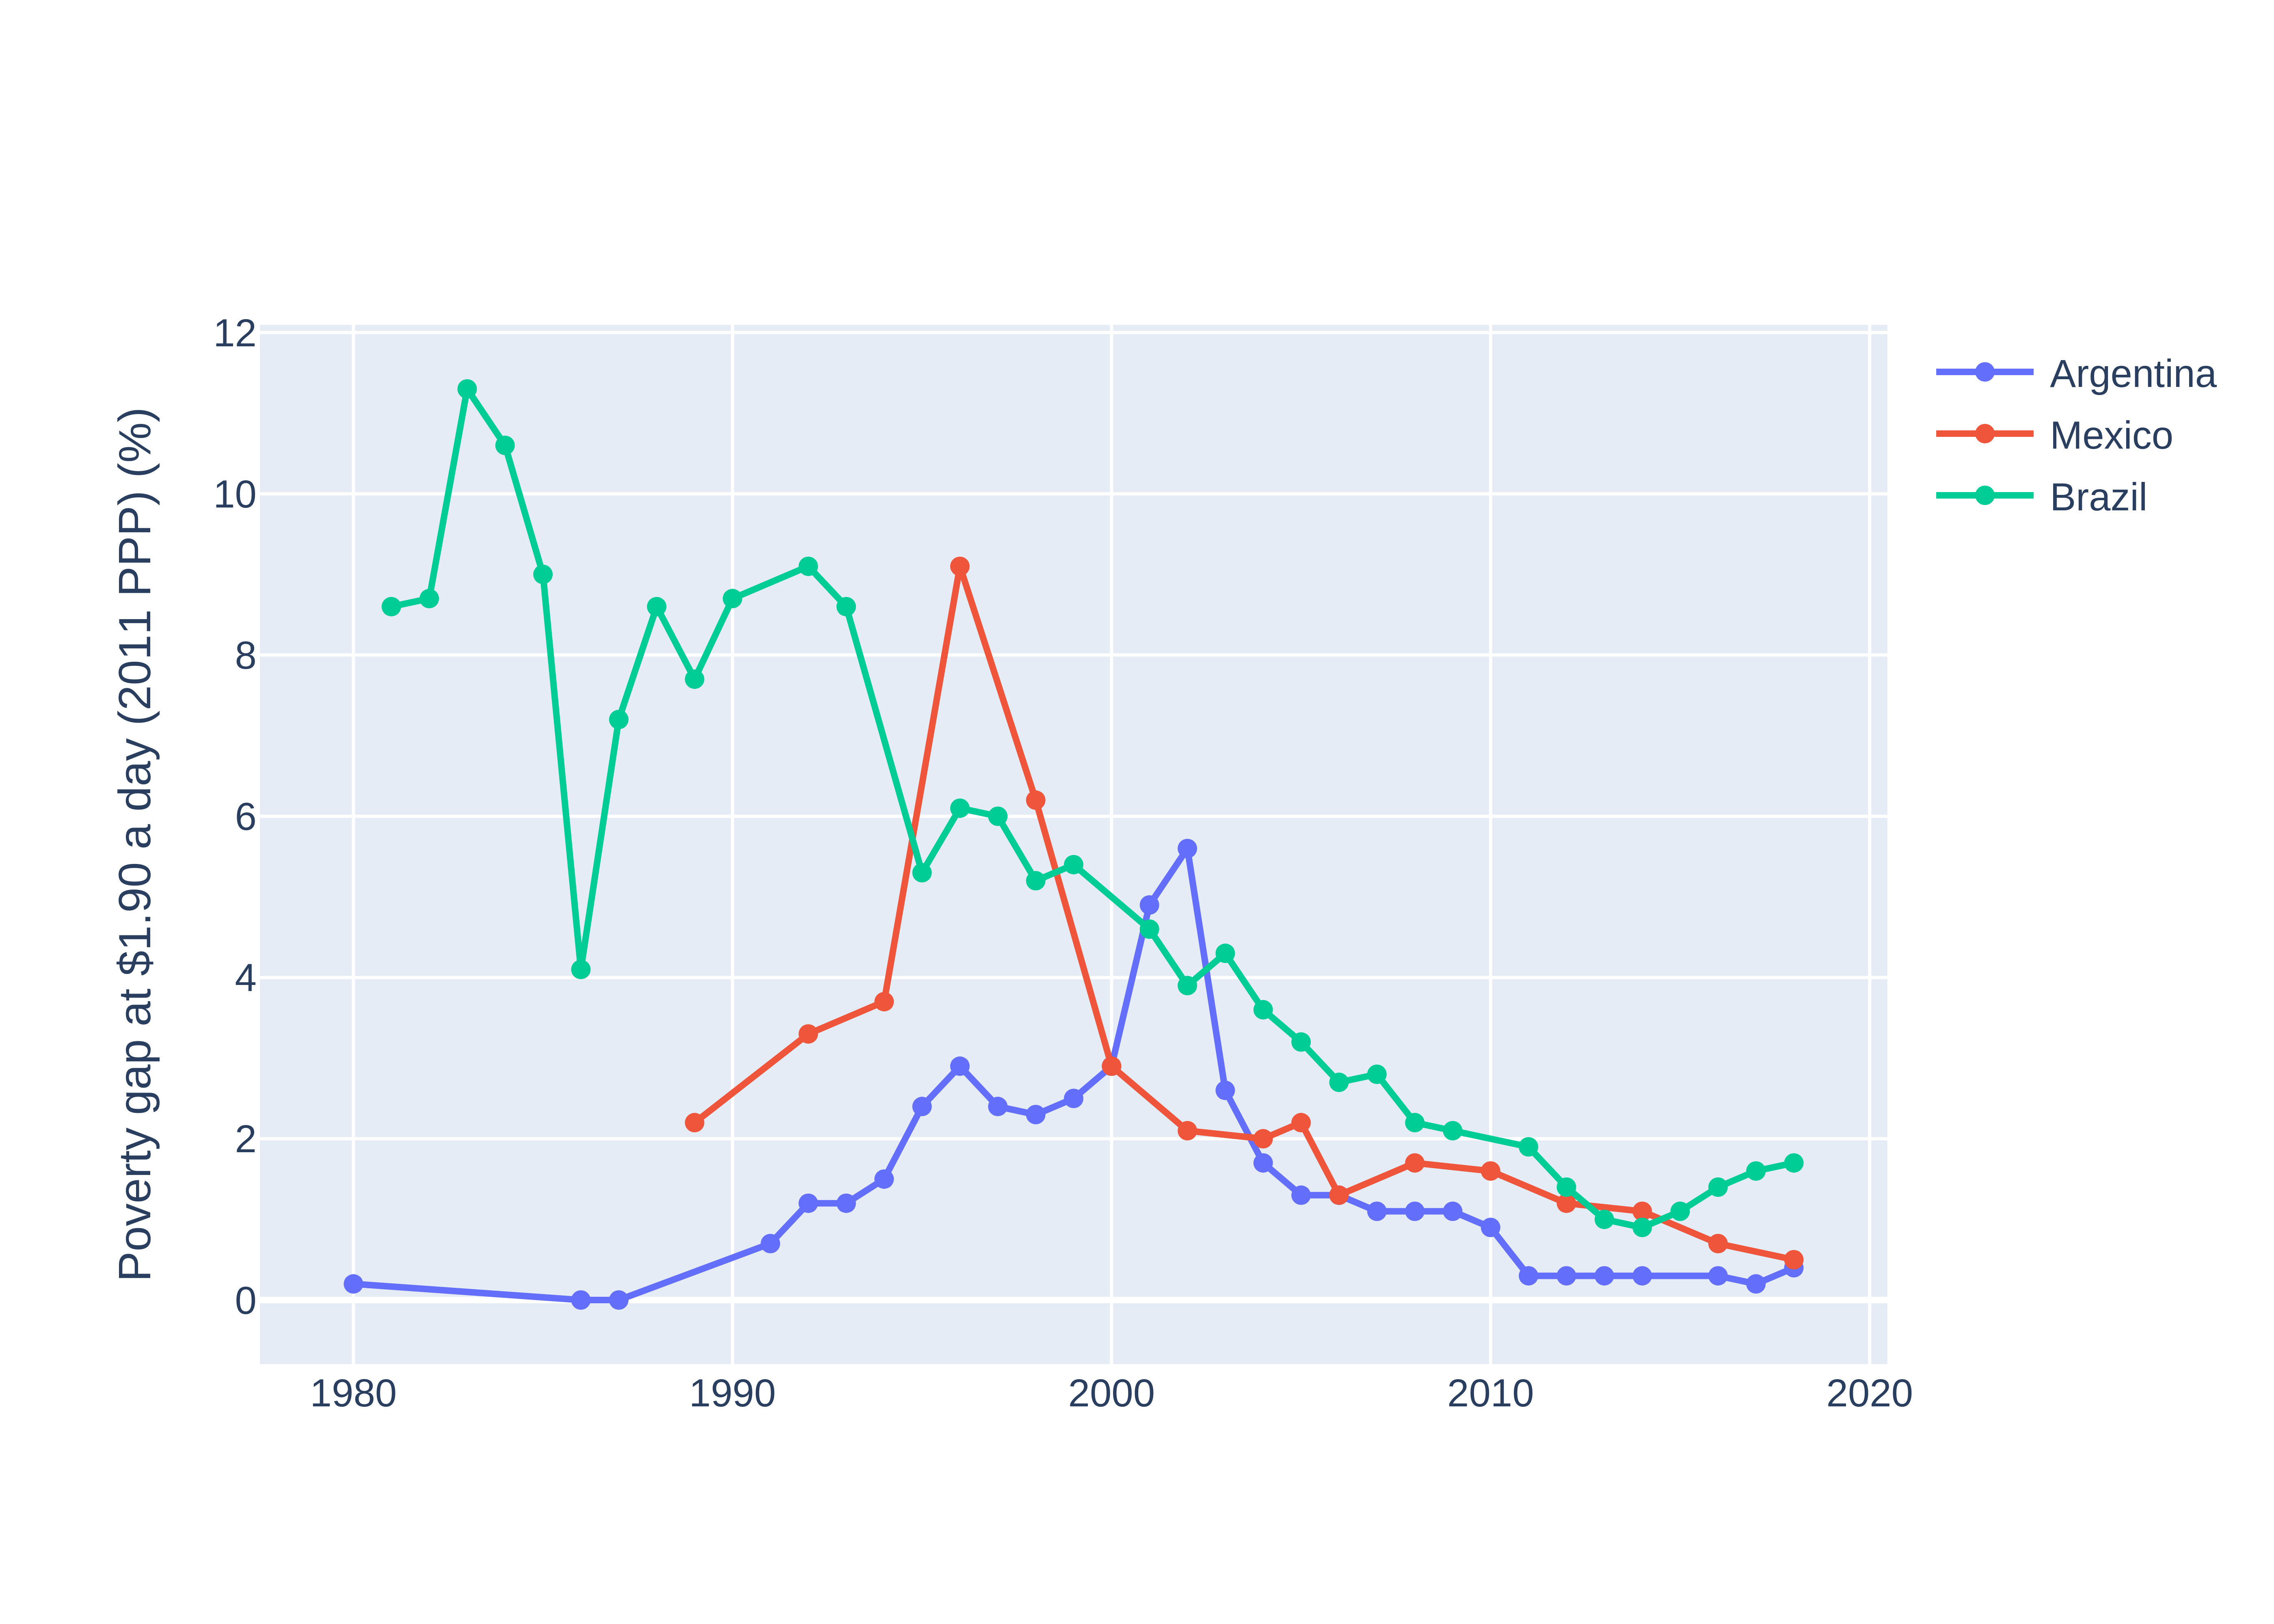
\includegraphics[width=7cm, height=7cm, keepaspectratio]{images/scatter_8.png}
				\end{center}
			\end{column}
		\end{columns}
	\end{frame}
	
	\section{Színek kezelése}
	
	\begin{frame}{}
		\tableofcontents[currentsection]
	\end{frame}
	
	\begin{frame}[fragile]{Alapértelmezett színezés folytonos változóval}
		\begin{columns}
			\begin{column}{.5\textwidth}
				A színezést a \texttt{px.scatter()} függvény hívásakor a \texttt{color} paraméterének állításával lehet elérni. Folytonos változó esetén a vászon jobb oldalán egy folytonos színskála fog megjelenni.\par\medskip
				\begin{lstlisting}[language=python]
fig = px.scatter(df, x=indicator, y='Country Name', color='Population, total')				
				\end{lstlisting}
			\end{column}
			\begin{column}{.5\textwidth}
				\begin{center}
					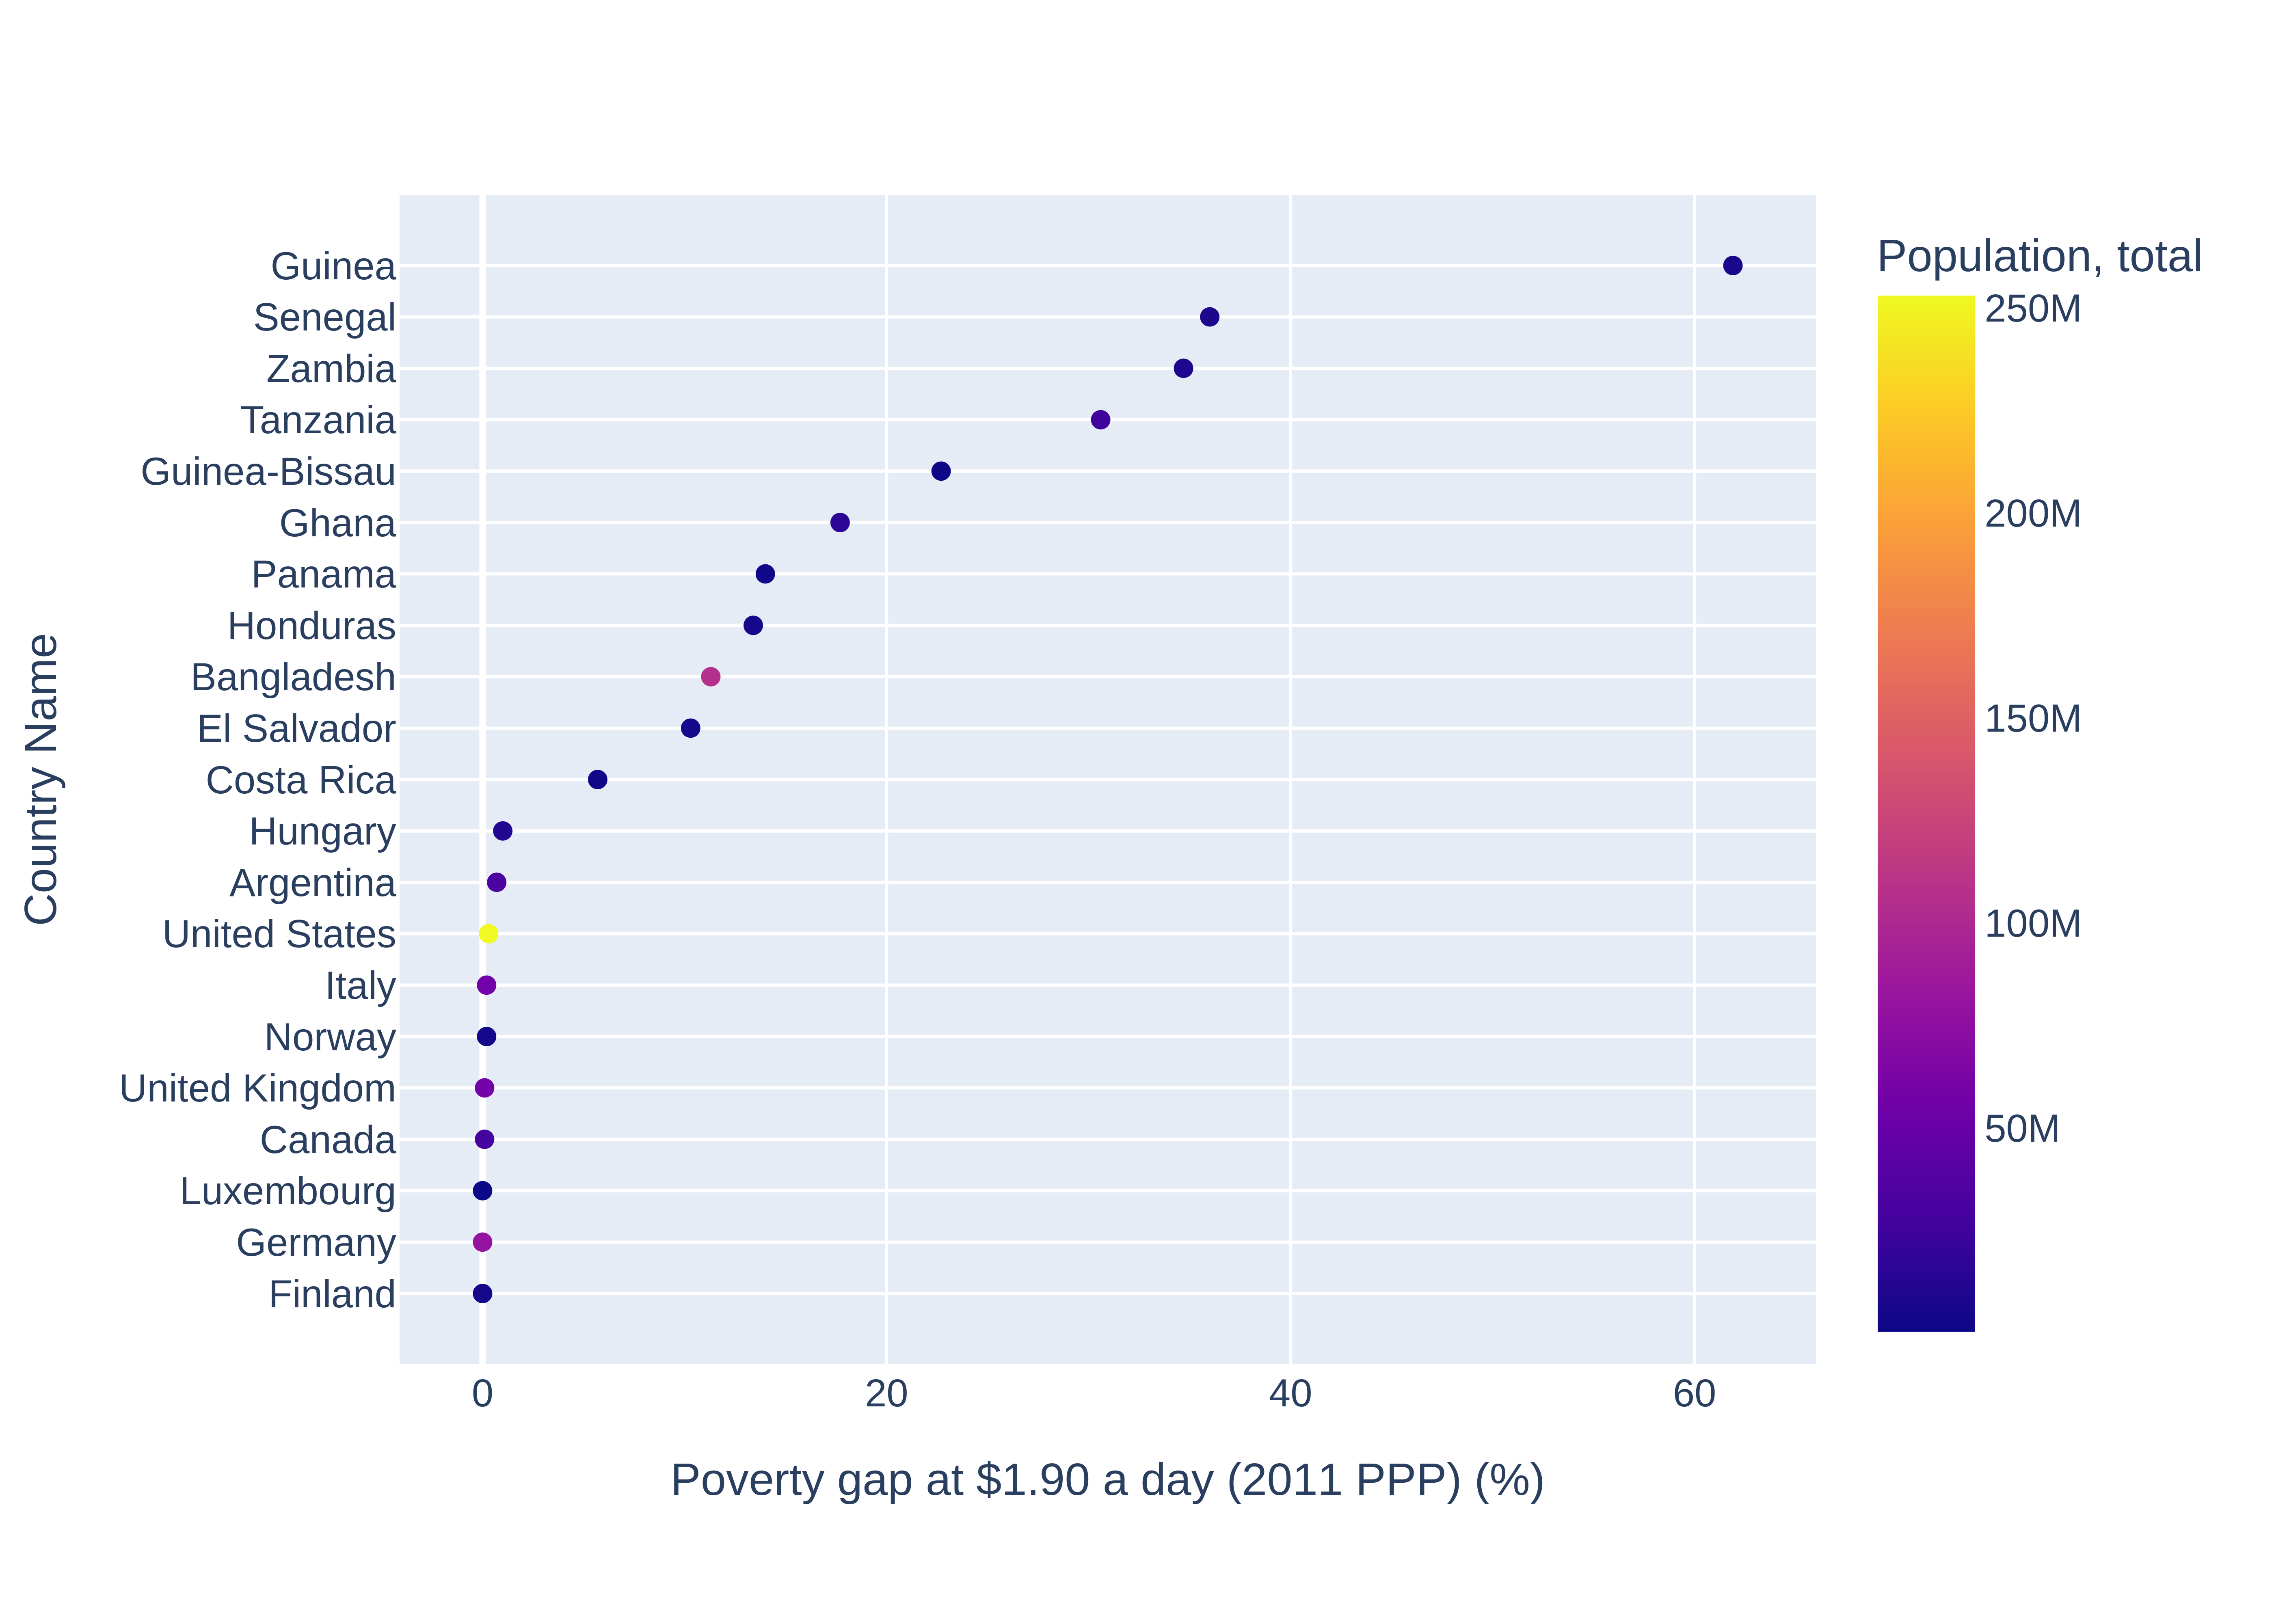
\includegraphics[width=7cm, height=7cm, keepaspectratio]{images/scatter_9.png}
				\end{center}
			\end{column}
		\end{columns}
	\end{frame}
	
	\begin{frame}[fragile]{Személyre szabott színezés folytonos változóval}
		\begin{columns}
			\begin{column}{.5\textwidth}
				A színskála megadható a \texttt{color\_continuous\_scale} paraméter állításával. A színskálák listája \href{https://plotly.com/python/builtin-colorscales/}{ezen a linken} érhető el.\par\medskip
				\begin{lstlisting}[language=python]
fig = px.scatter(df, x=indicator, y='Country Name', color='Population, total', color_continuous_scale='RdBu')				
				\end{lstlisting}
			\end{column}
			\begin{column}{.5\textwidth}
				\begin{center}
					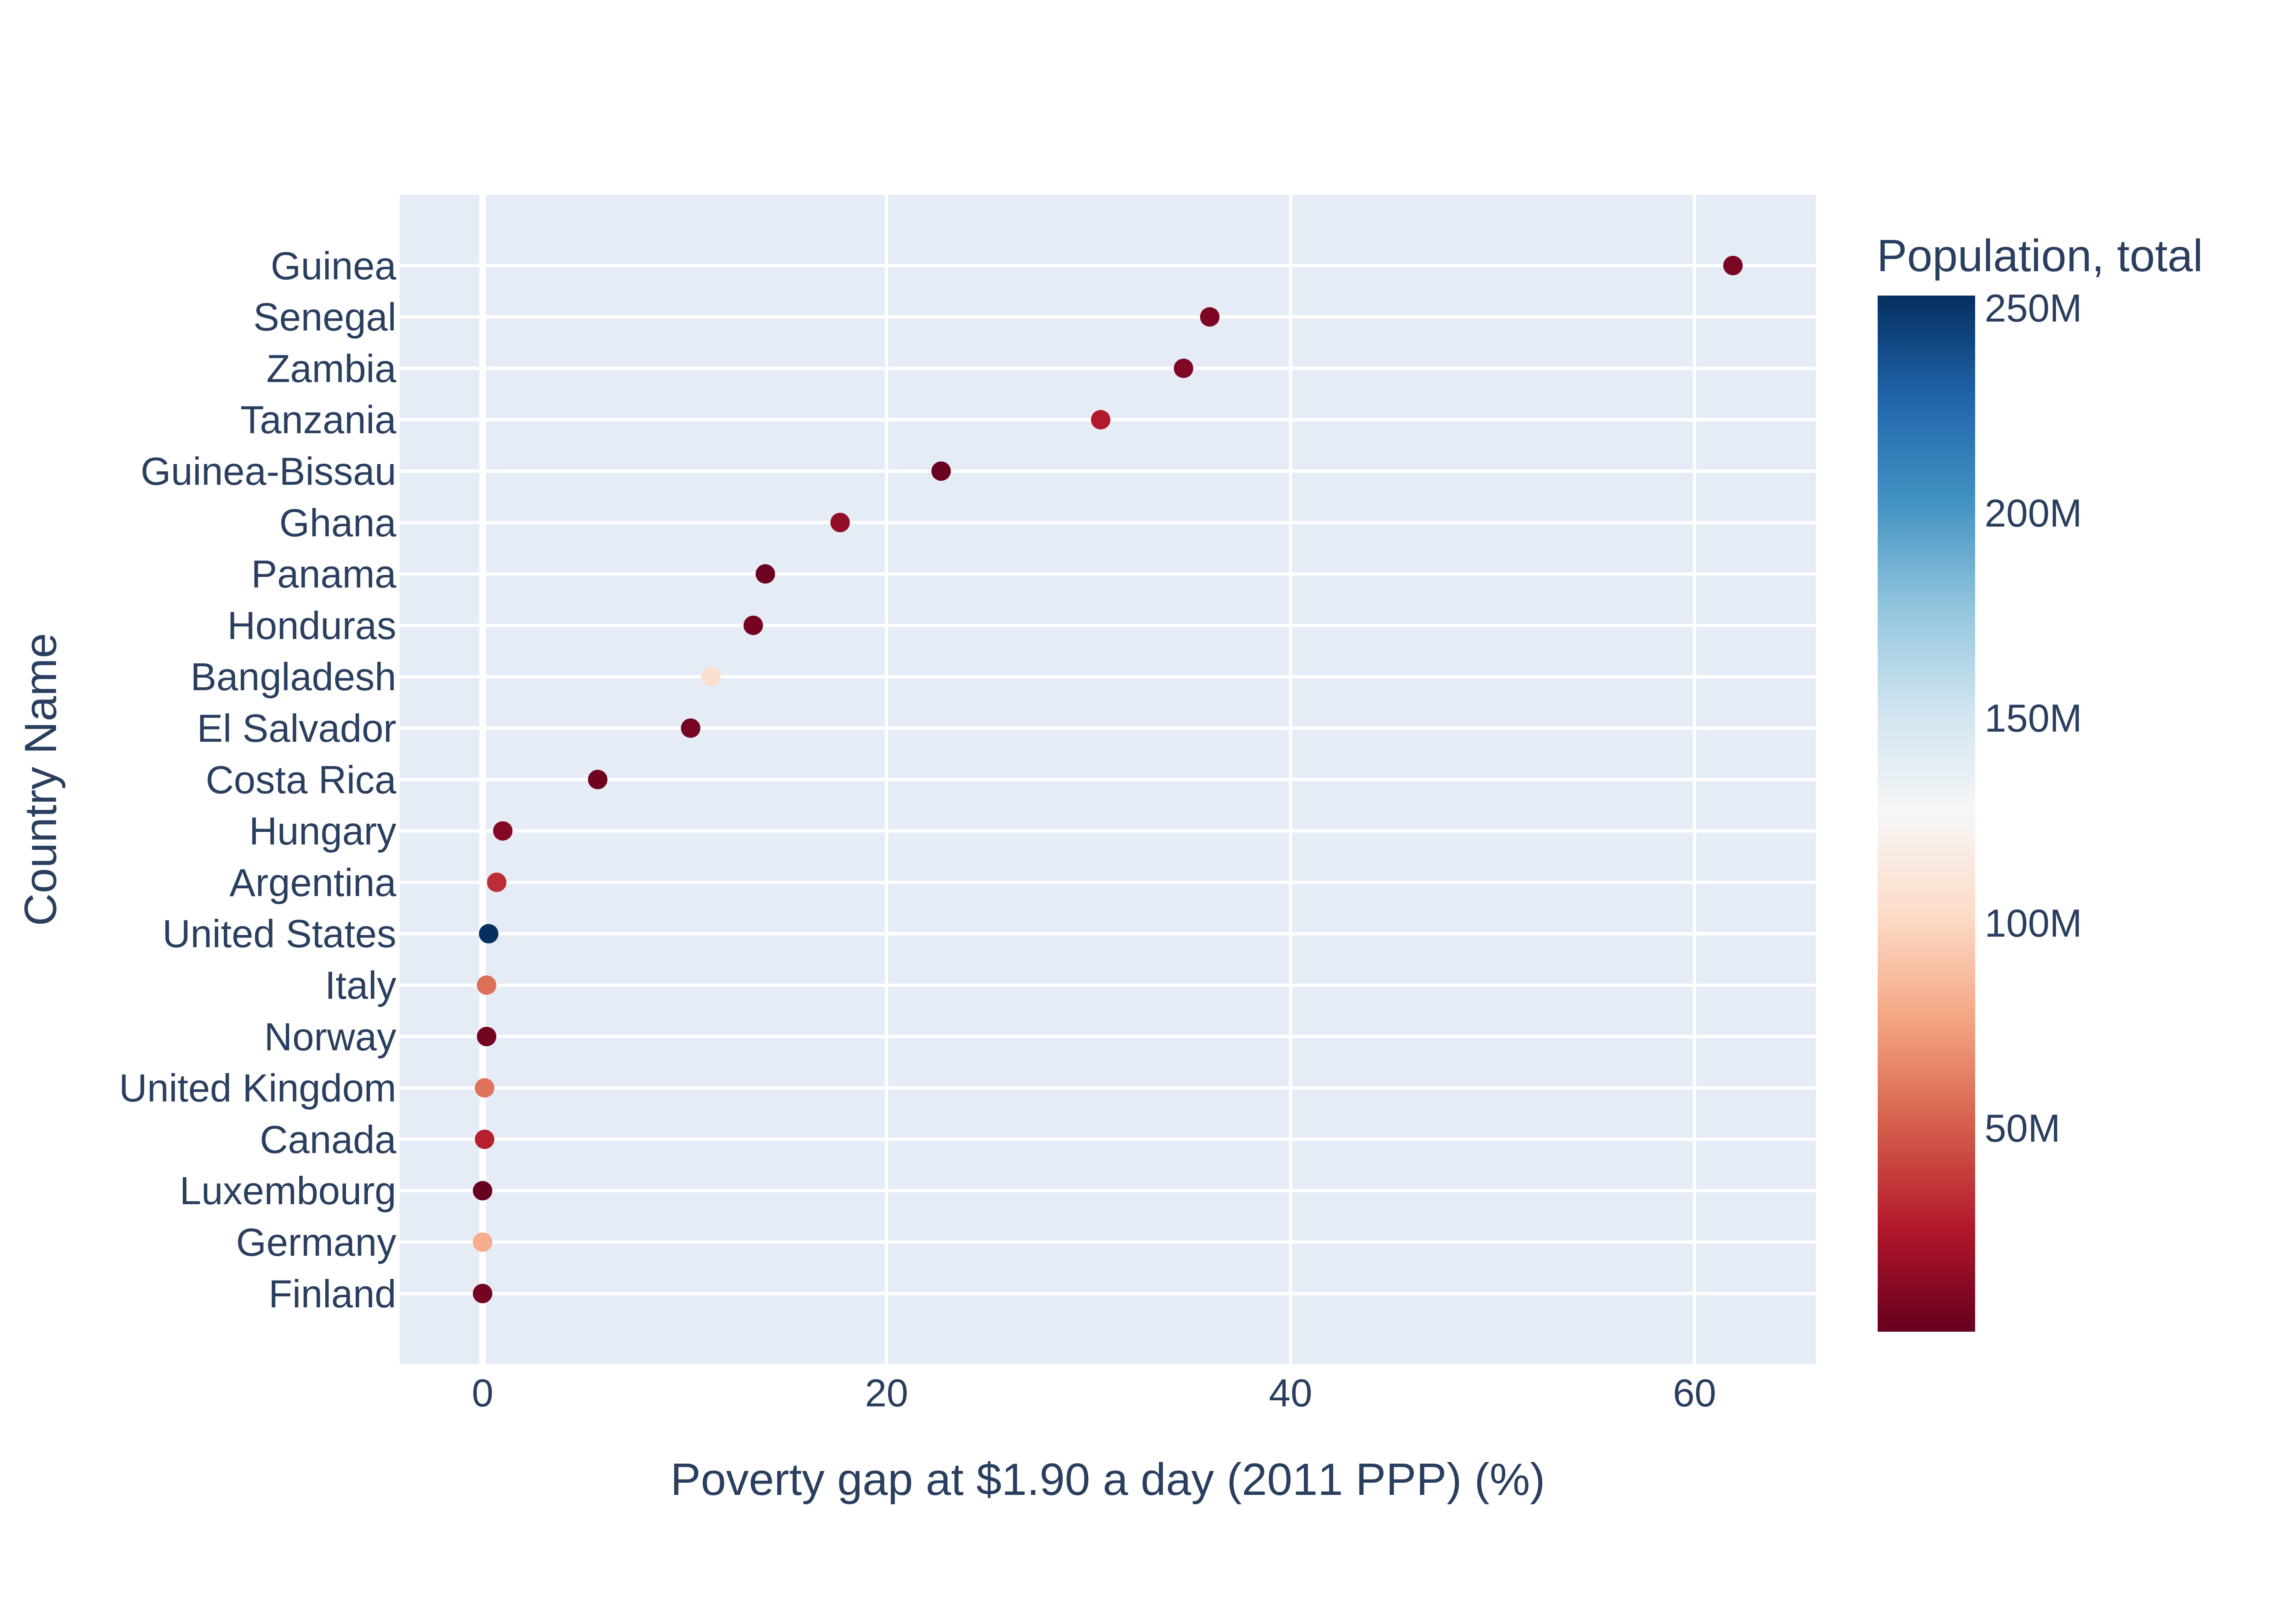
\includegraphics[width=7cm, height=7cm, keepaspectratio]{images/scatter_10.png}
				\end{center}
			\end{column}
		\end{columns}
	\end{frame}
	
	\begin{frame}[fragile]{Színek diszkrét változókkal}
		\begin{columns}
			\begin{column}{.5\textwidth}
				Ha a diagramon ábrázolt függő változó diszkrét, nem egy színskála jön létre, hanem a diagram jobb oldalán a lehetséges kategóriák lesznek felsorolva, amelyek közül kattintással lehet kiválasztani a megjelenítendő nyomot.\par\medskip
				\begin{lstlisting}[language=python]
fig = px.scatter(
	df,
	x=indicator,
	y='Country Name',
	color='Income Group',
	...
)				
				\end{lstlisting}
			\end{column}
			\begin{column}{.5\textwidth}
				\begin{center}
					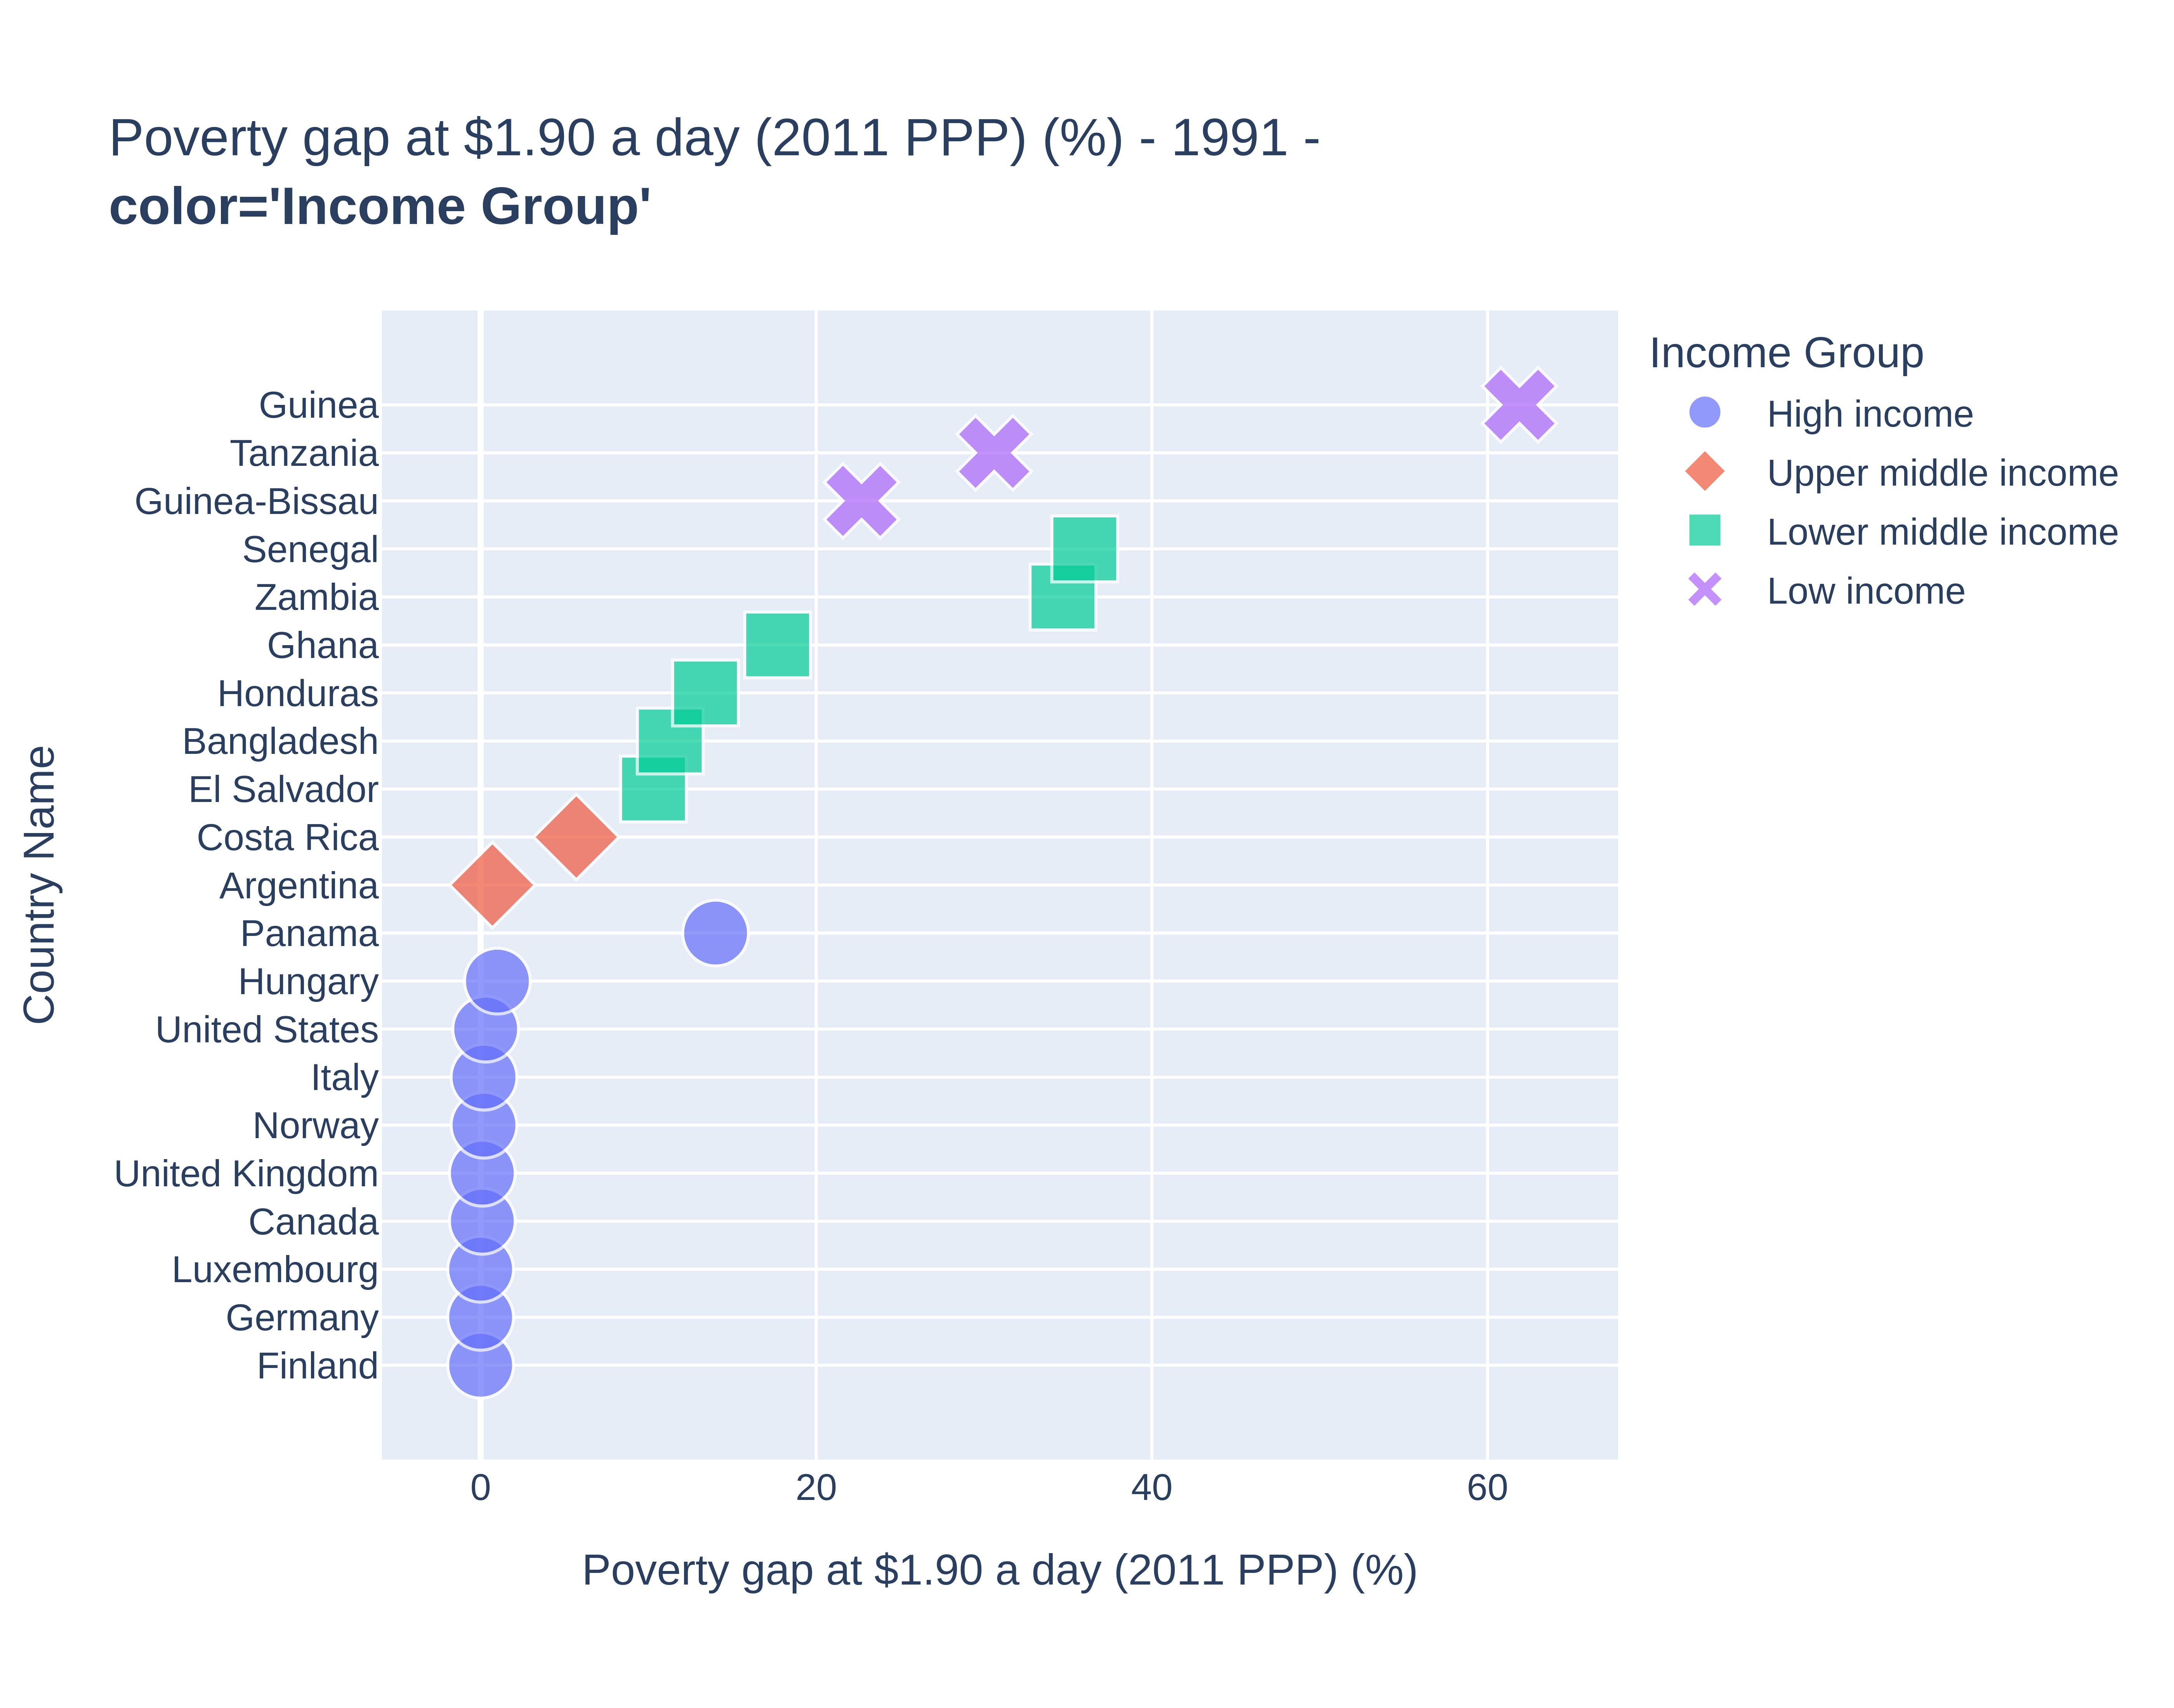
\includegraphics[width=7cm, height=7cm, keepaspectratio]{images/scatter_11.png}
				\end{center}
			\end{column}
		\end{columns}
	\end{frame}
	
	\begin{frame}[fragile]{Egyéni színek diszkrét változókkal}
		\begin{columns}
			\begin{column}{.5\textwidth}
				A \texttt{color\_discrete\_sequence} paraméter egy listát fogad, ahol minden elem egy színnevet tartalmazó szöveges érték.\par\medskip
				\begin{lstlisting}[language=python]
fig = px.scatter(
	df,
	x=indicator,
	y='Country Name',
	color='Income Group',
	symbol='Income Group',
	color_discrete_sequence=['chocolate', 'teal', 'olive', 'black'],
	...
)
				\end{lstlisting}
			\end{column}
			\begin{column}{.5\textwidth}
				\begin{center}
					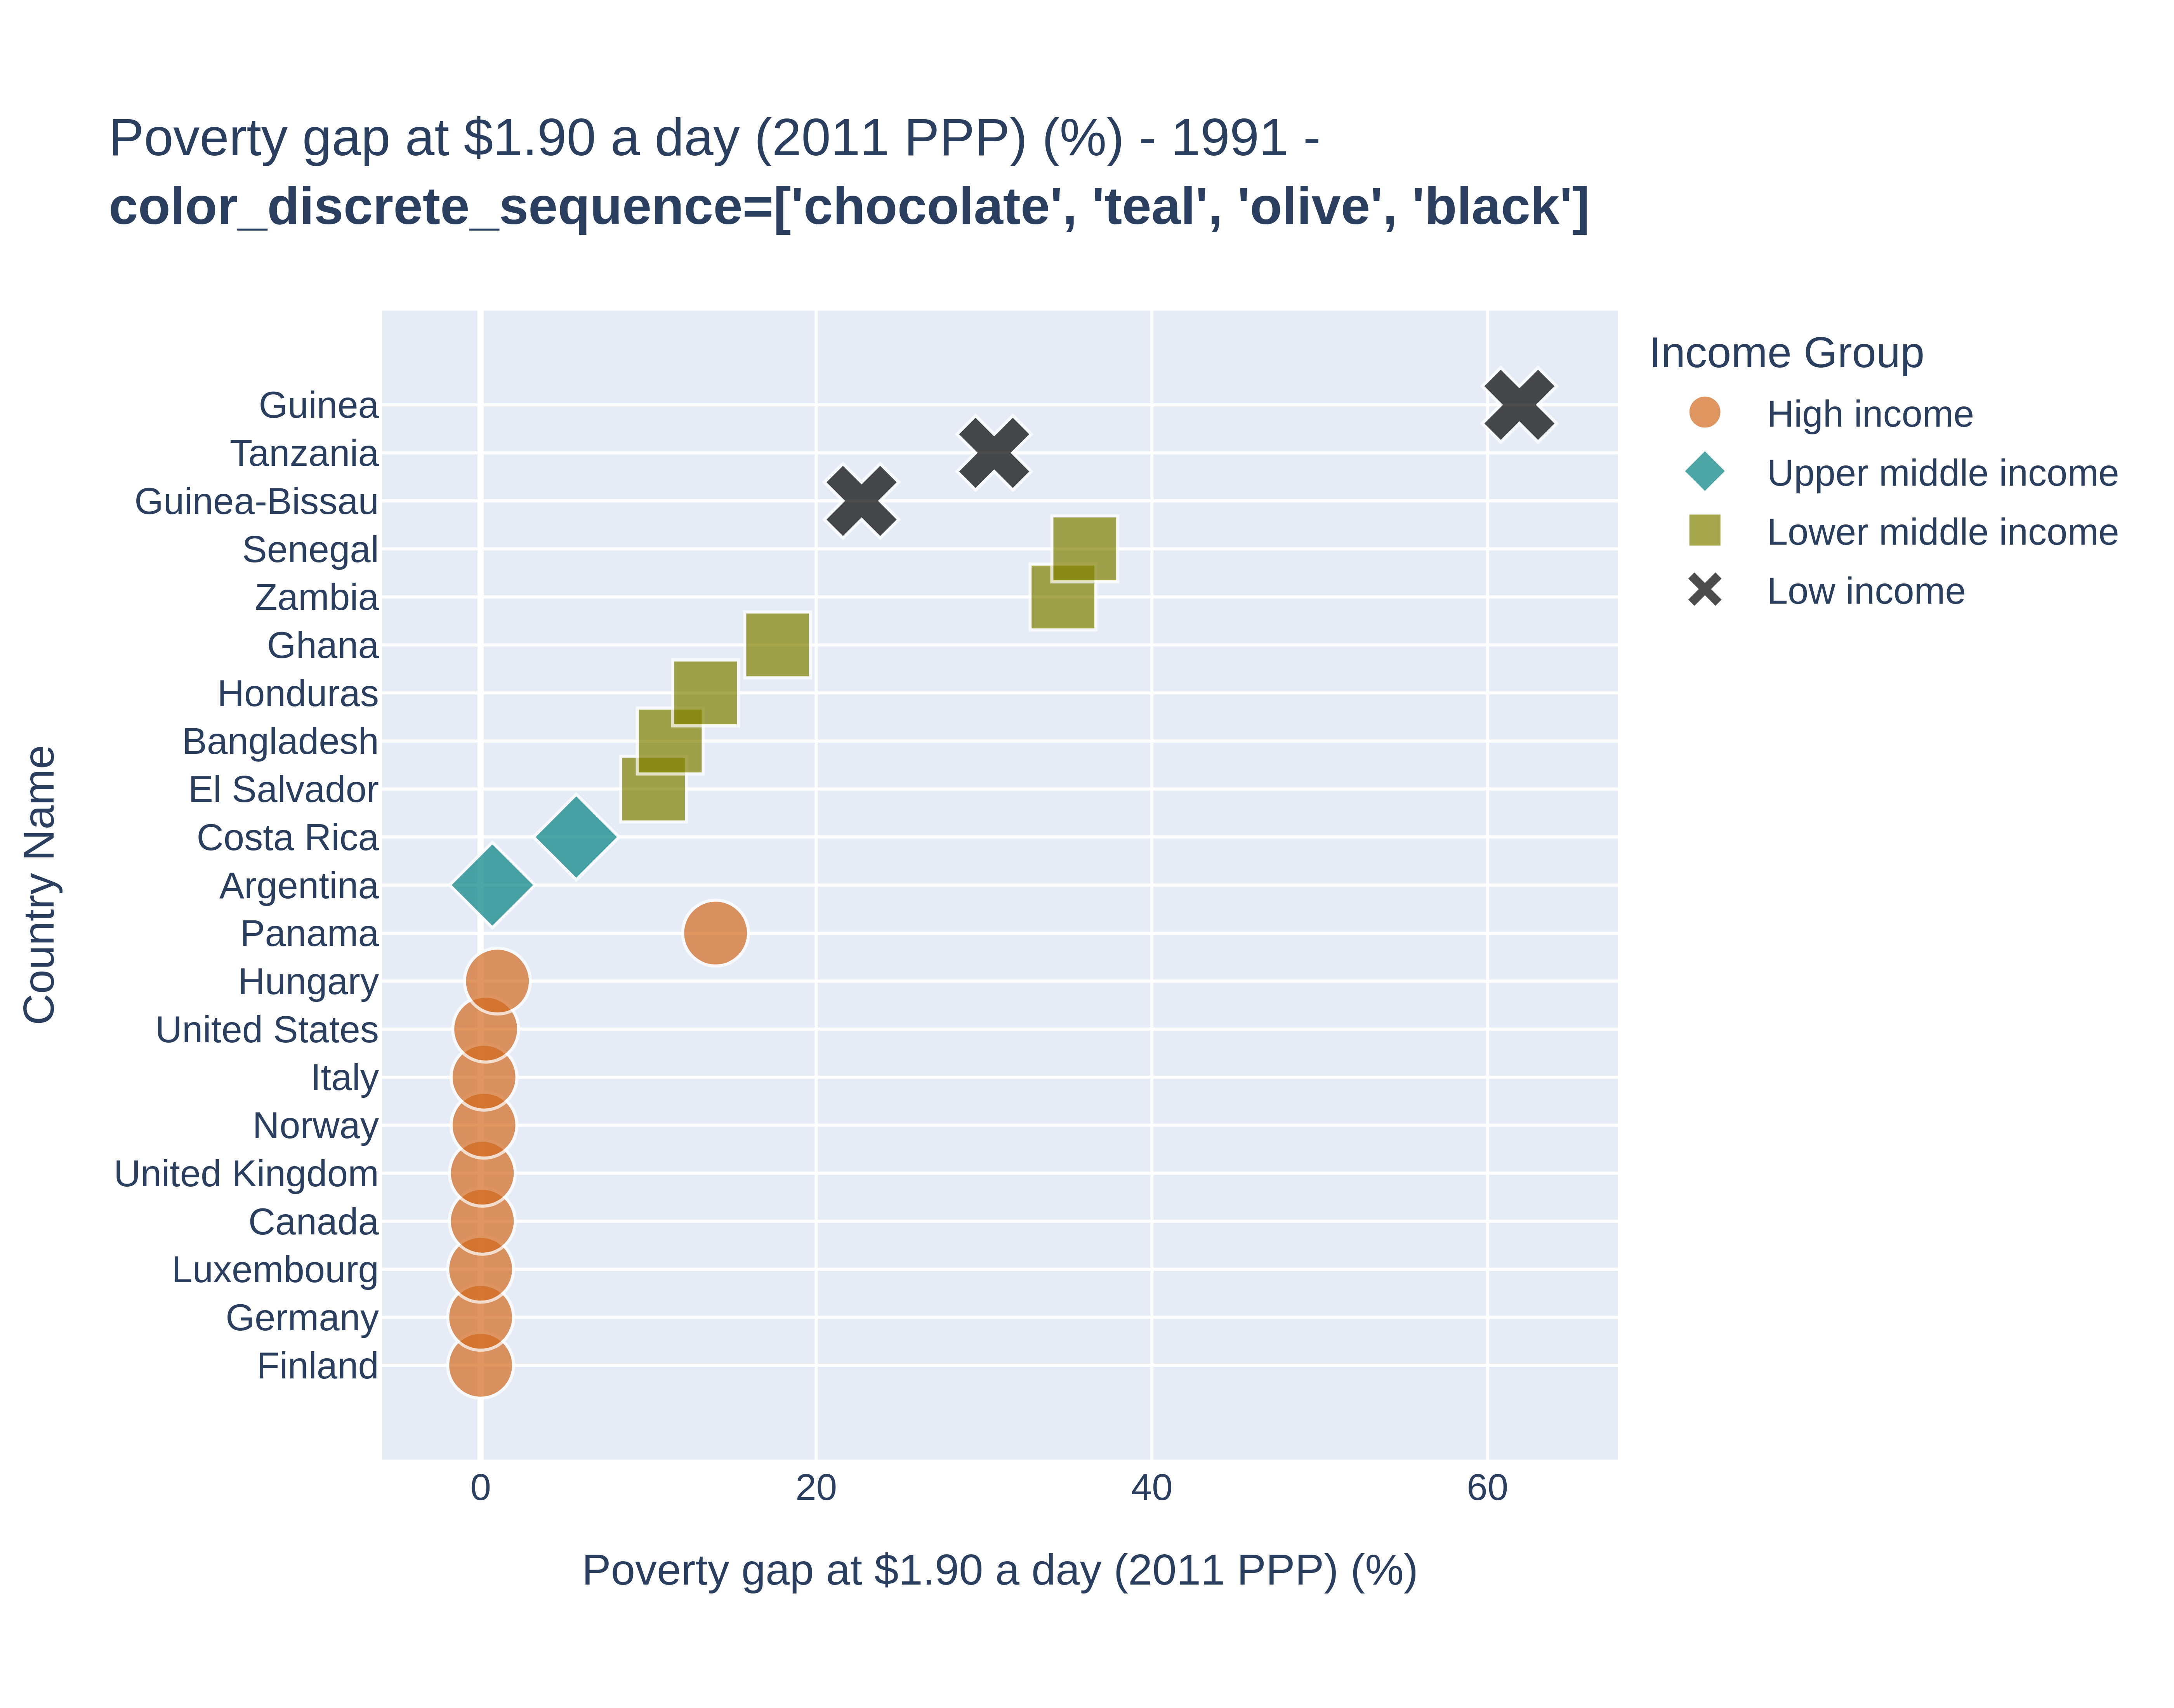
\includegraphics[width=7cm, height=7cm, keepaspectratio]{images/scatter_12.png}
				\end{center}
			\end{column}
		\end{columns}
	\end{frame}
	
	\section{Kiugró értékek}
	
	\begin{frame}{}
		\tableofcontents[currentsection]
	\end{frame}
	
	\begin{frame}{Kiugró értékek a gyakorlatban}
		\begin{columns}
			\begin{column}{.5\textwidth}
				A következő példában egyetlen outlier érték, Kína a maga 1.4 milliárd lélekszámával az összes többi országot egy kis területbe szorítja a diagram bal oldalán.\par\medskip
				A következő fejezet azzal fog foglalkozni, hogy hogyan lehet ilyen jelenségeket kezelni.
			\end{column}
			\begin{column}{.5\textwidth}
				\begin{center}
					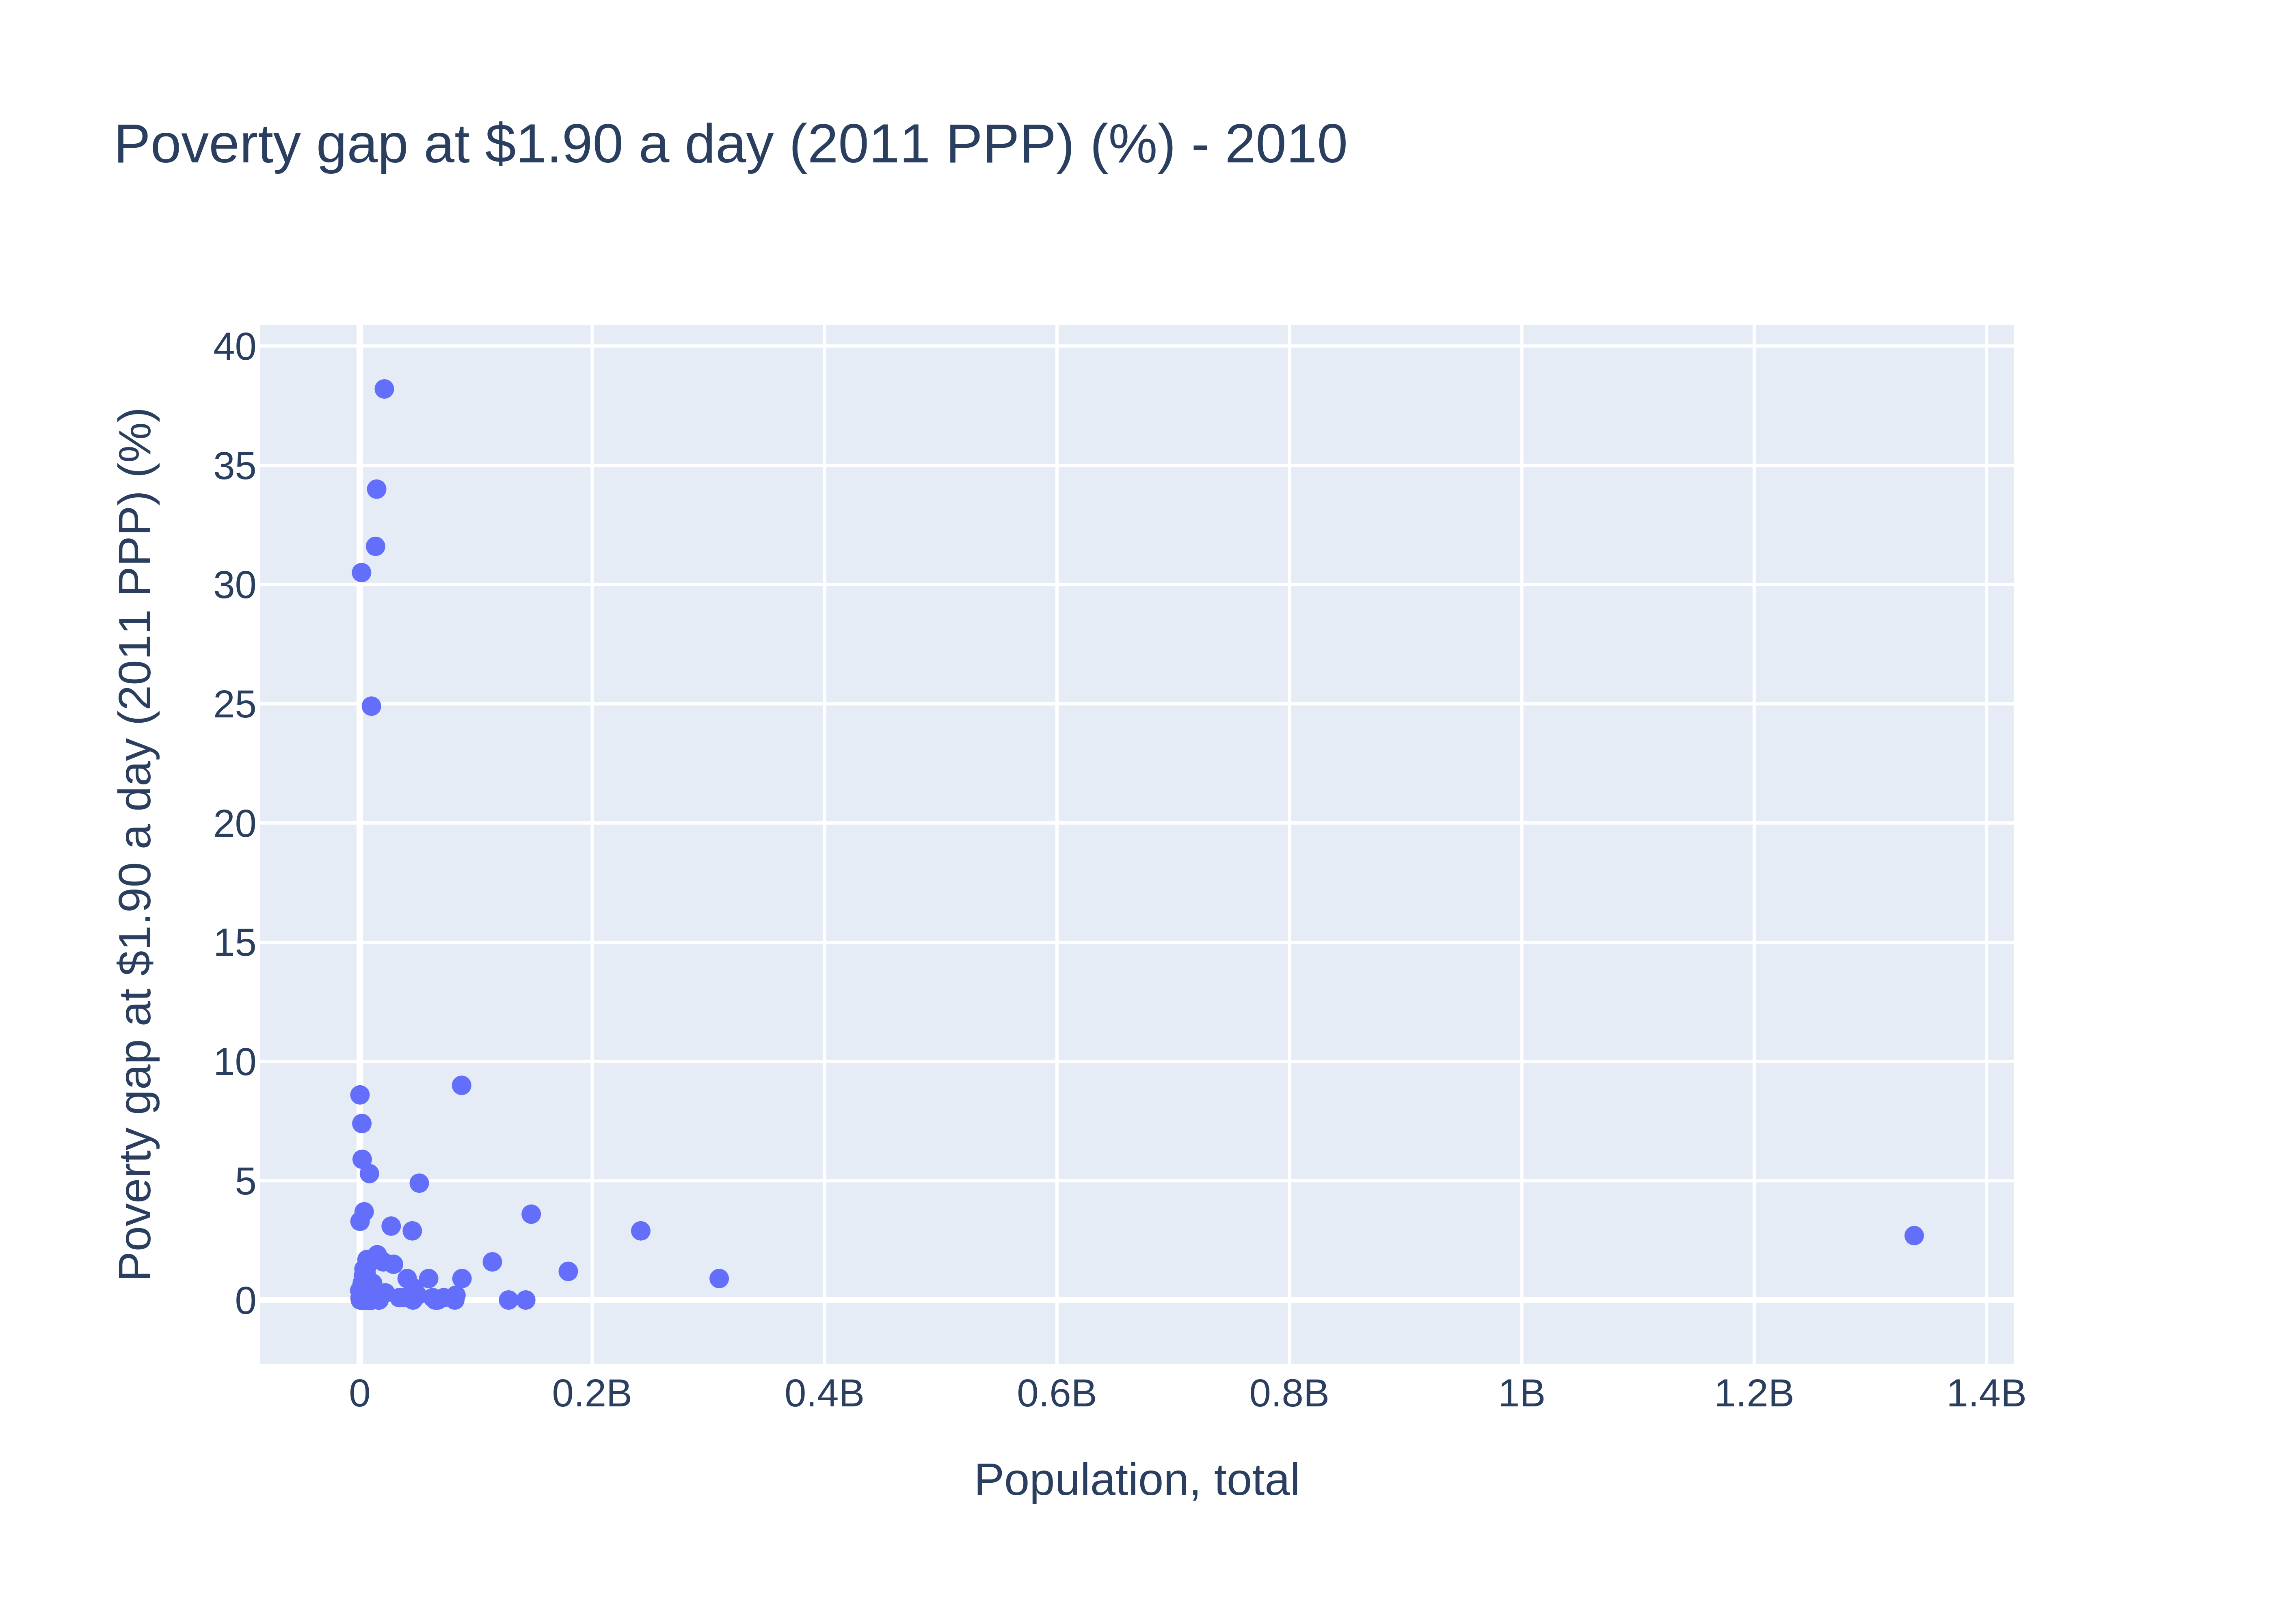
\includegraphics[width=7cm, height=7cm, keepaspectratio]{images/scatter_13.png}
				\end{center}
			\end{column}
		\end{columns}
	\end{frame}
	
	\begin{frame}[fragile]{Markerek áttetszőségének és méretének állítása}
		\begin{columns}
			\begin{column}{.5\textwidth}
				Az \texttt{opacity} paraméter egy $\left[0,1\right]$ intervallumba eső tizedes törtet vár el paraméterül. A 0 érték egy teljesen áttetsző, az 1 pedig egy teljesen átlátszatlan markert fog eredményezni.\par\medskip
				Mivel a markerek nagyon kicsik, a \texttt{size} paraméter növelésével jobban láthatóvá lehet őket tenni.
			\end{column}
			\begin{column}{.5\textwidth}
				\begin{center}
					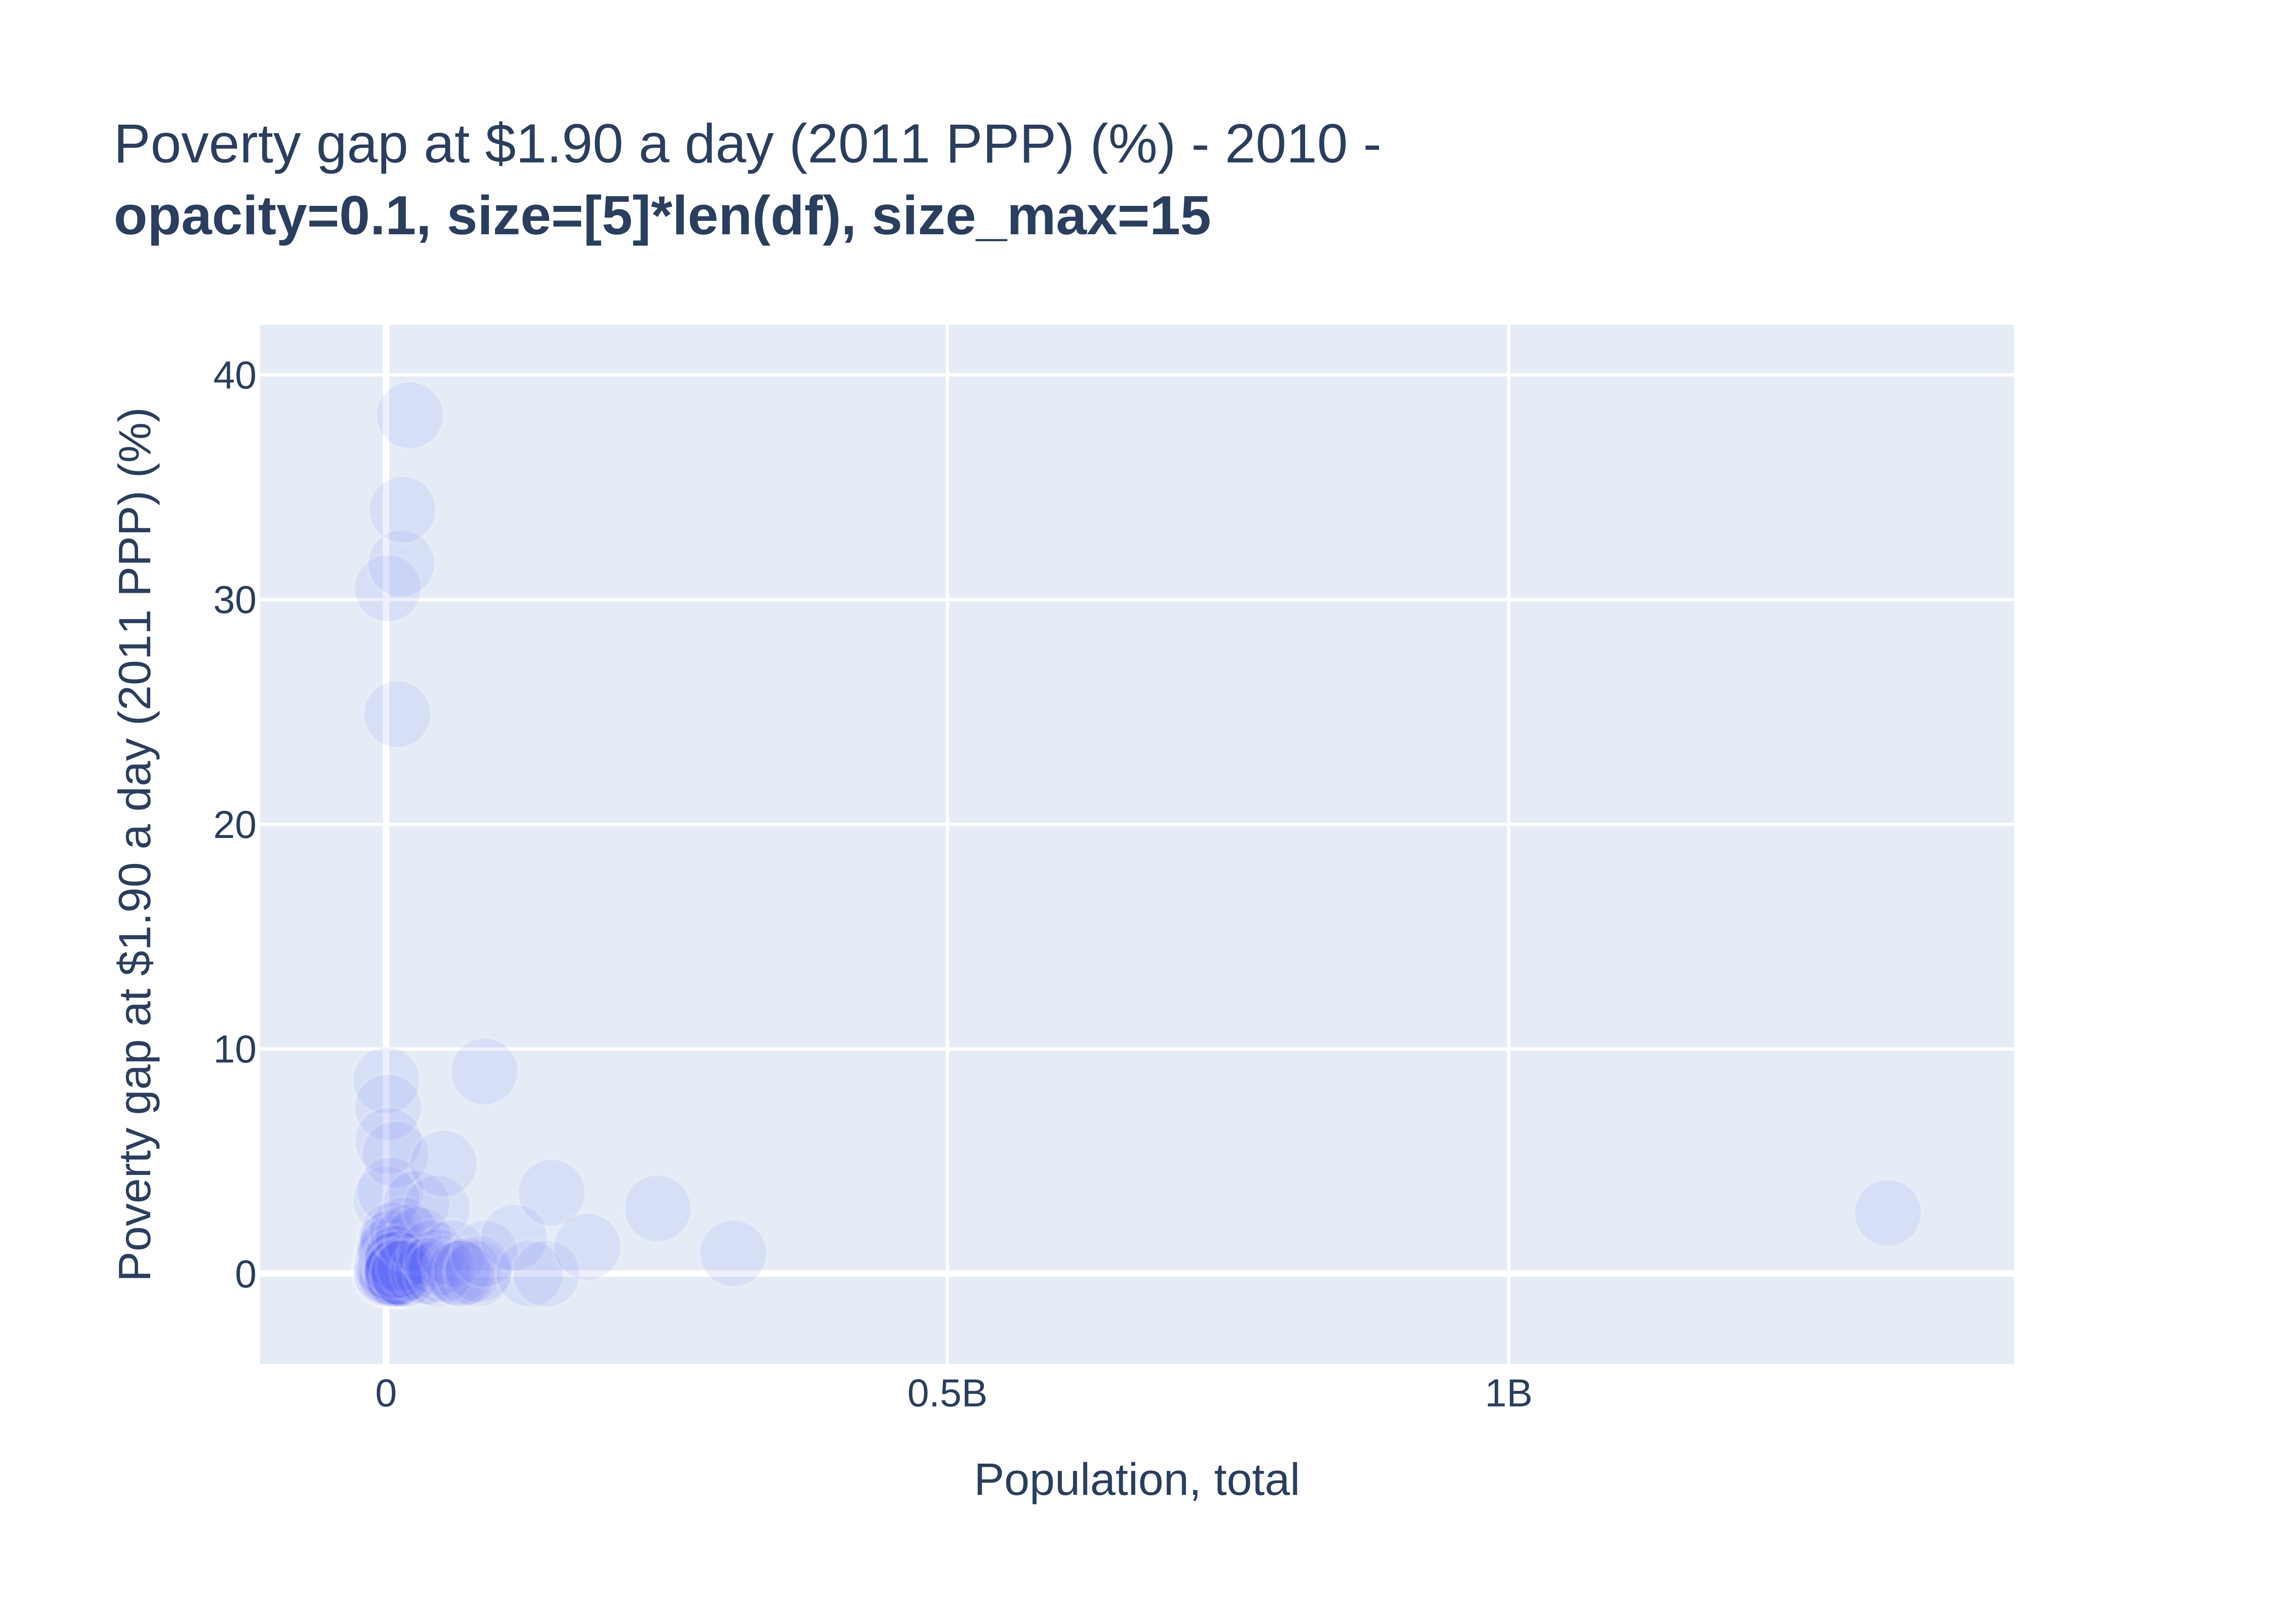
\includegraphics[width=7cm, height=7cm, keepaspectratio]{images/scatter_14.png}
				\end{center}
			\end{column}
		\end{columns}
	\end{frame}
	
	\begin{frame}{Logaritmikus skála használata}
		\begin{columns}
			\begin{column}{.5\textwidth}
				A logaritmikus skála olyan skála, amelyen az értékek nem egyenletesen, hanem logaritmikus arányban vannak elosztva. Például egy 10-es alapú logaritmikus skálán a jelölések 1, 10, 100, 1000 stb. lehetnek.\par\medskip
				Logaritmikus skálát egy plotly diagramon a \texttt{log\_x} paraméter bekapcsolásával lehet létrehozni. 
			\end{column}
			\begin{column}{.5\textwidth}
				\begin{center}
					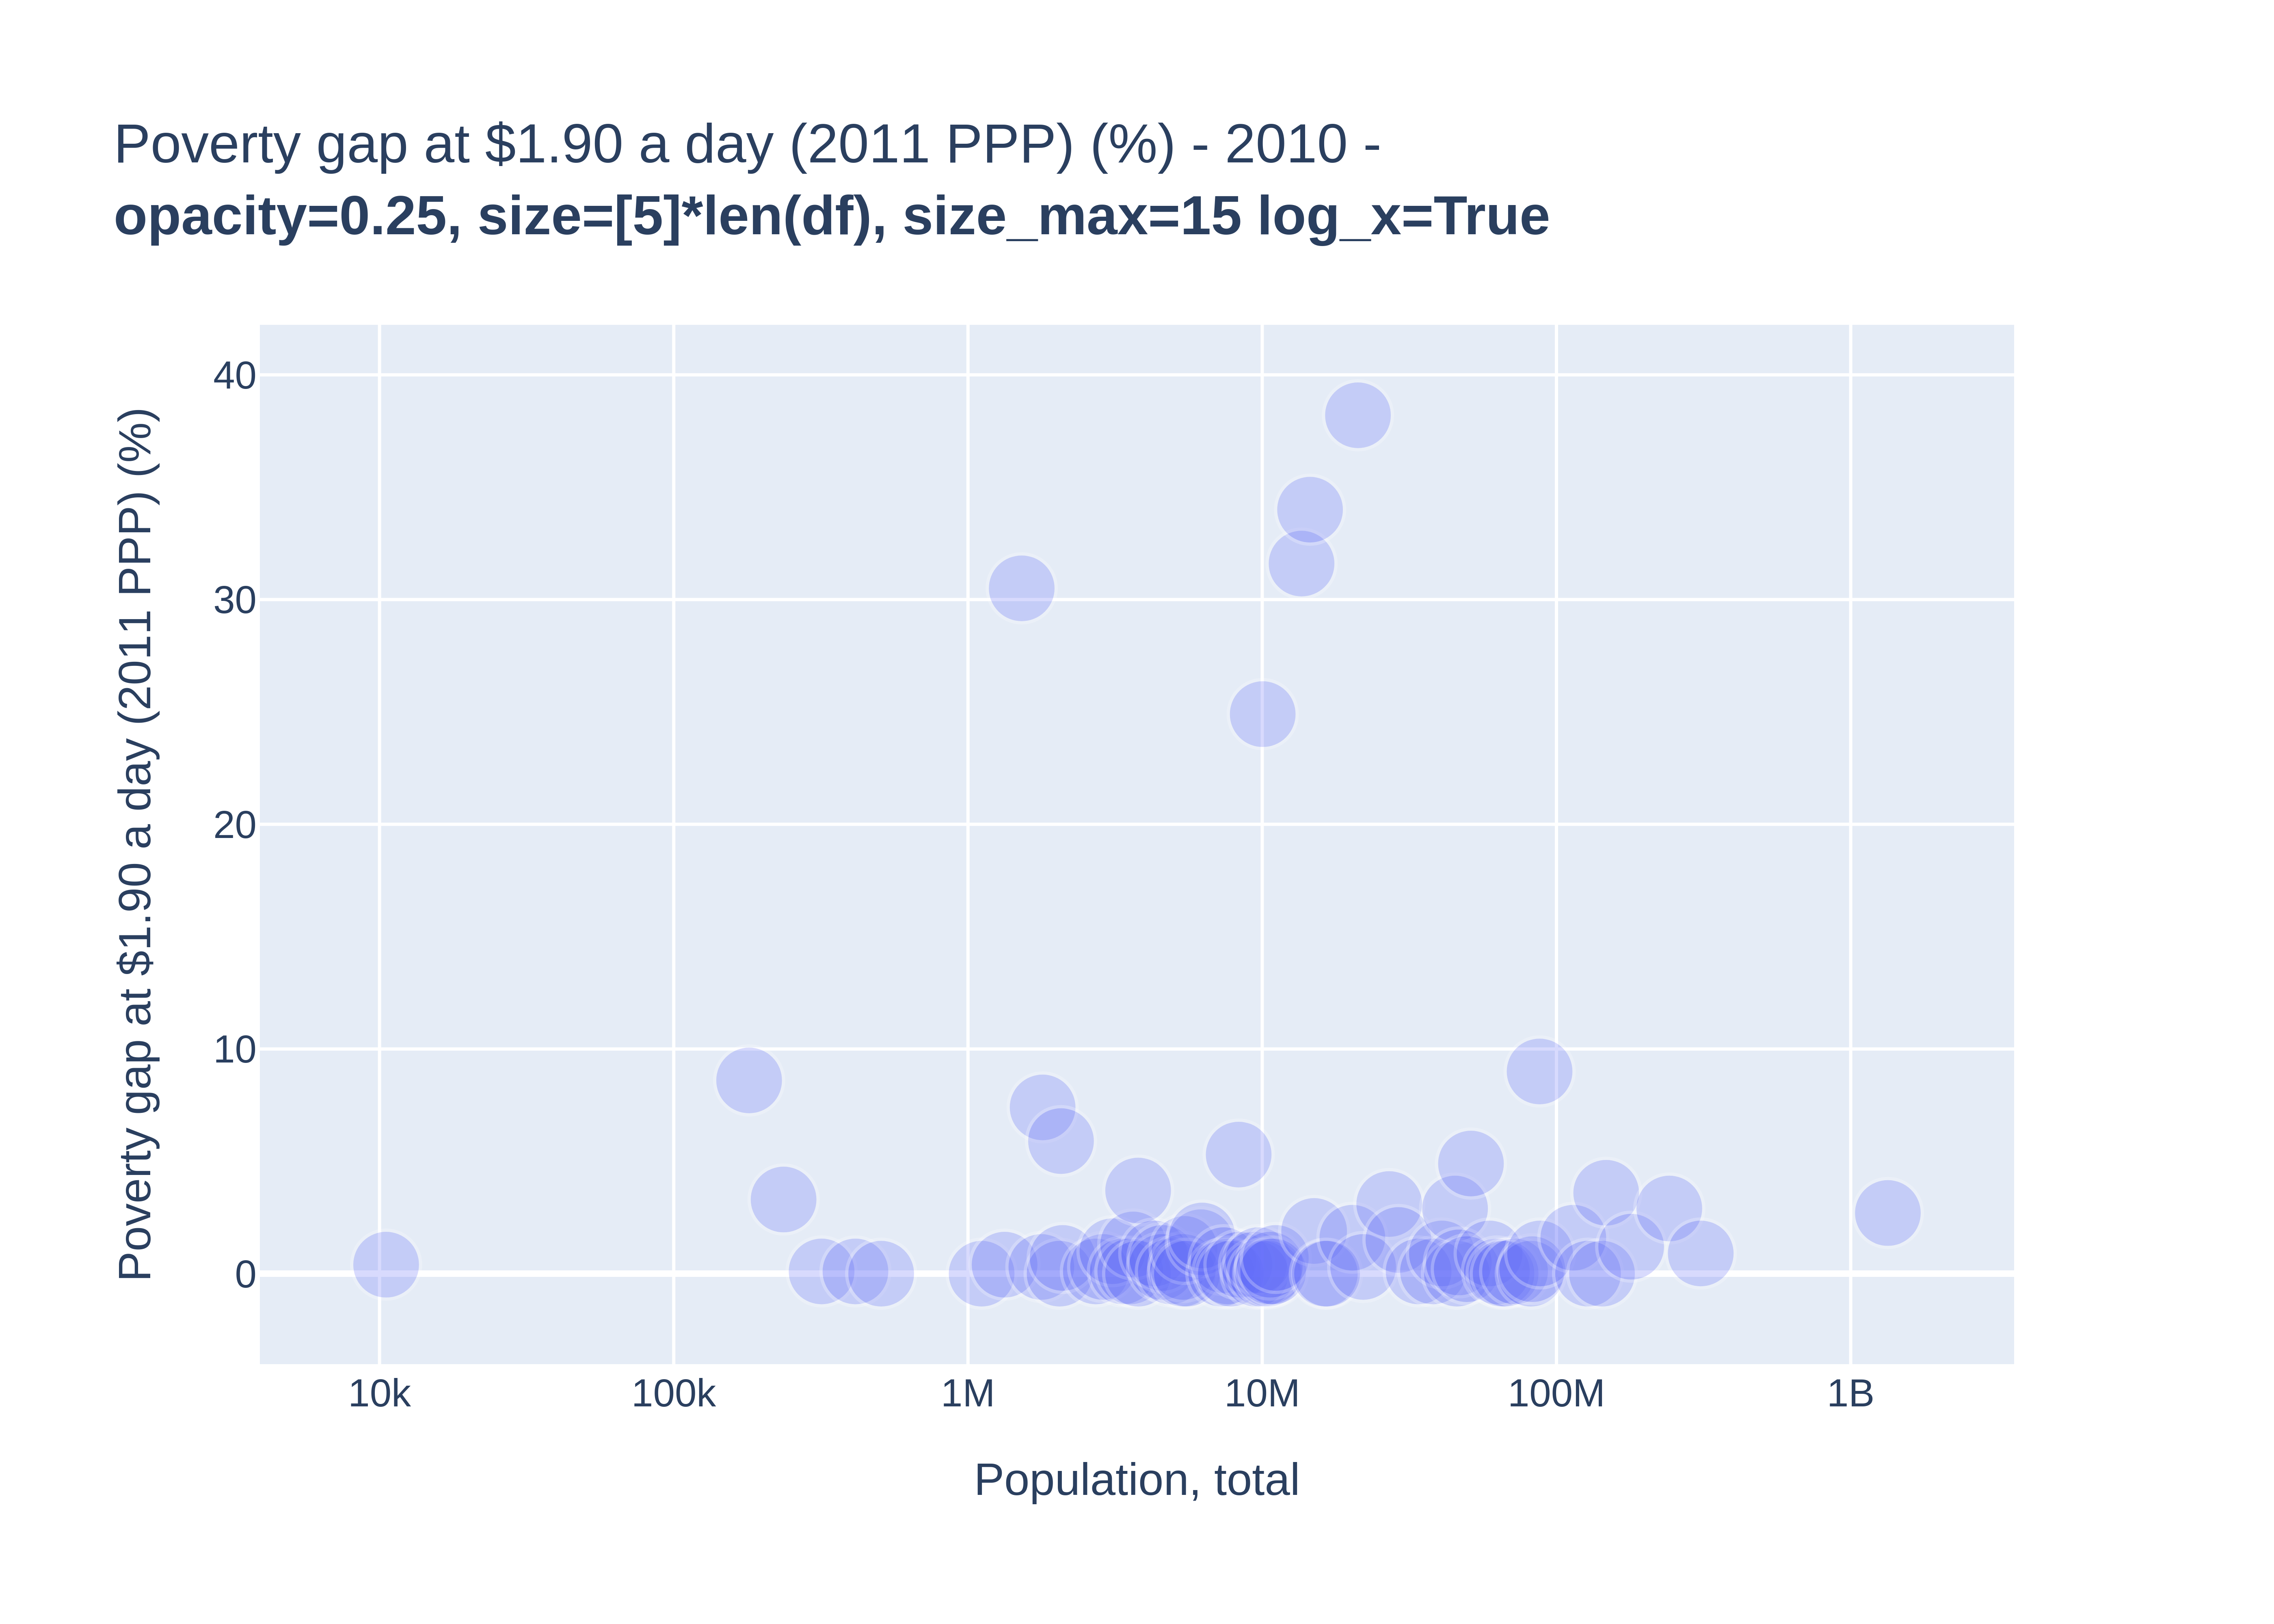
\includegraphics[width=7cm, height=7cm, keepaspectratio]{images/scatter_15.png}
				\end{center}
				\end{column}
		\end{columns}
	\end{frame}
	
	\section{Csúszkák}
	
	\begin{frame}{}
		\tableofcontents[currentsection]
	\end{frame}
	
	\begin{frame}[fragile]{Dash csúszkák}
		A \texttt{Slider} és \texttt{RangeSlider} komponensek körök, amelyeket a felhasználók húzhatnak egy érték beállításához, és folyamatos vagy kategorikus értékekhez is használhatók.\par\medskip
		A \texttt{Slider} egyetlen értéket állít, míg a \texttt{RangeSlider} komponensen két csúszka szerepel, és az ezek által határolt tartományt adja meg. 
		\begin{columns}
			\begin{column}{.5\textwidth}
				\begin{lstlisting}[language=python]
app = dash.Dash(__name__)
app.layout = html.Div([
	dcc.Slider(
		id='slider',
		min=0,
		max=20
	)
])
app.run_server(mode='inline')				
				\end{lstlisting}
			\end{column}
			\begin{column}{.5\textwidth}
				\begin{center}
					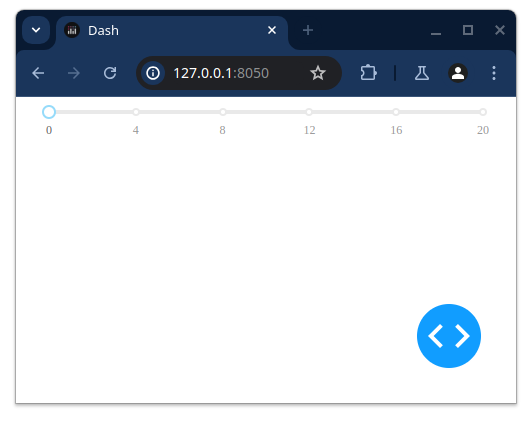
\includegraphics[width=4cm, height=7cm, keepaspectratio]{images/scatter_16.png}
				\end{center}
			\end{column}
		\end{columns}
	\end{frame}
	
	\begin{frame}[fragile]{\texttt{Slider} komponensek paraméterei}
		\begin{columns}
			\begin{column}{.5\textwidth}
				\begin{itemize}
					\item \texttt{min}: A csúszka minimum értéke
					\item \texttt{max}: A csúszka maximum értéke
					\item \texttt{step}: A legkisebb állítható lépték
					\item \texttt{dots}: Szerepeljenek-e markerek a csúszkán
					\item \texttt{included}: Ha az értéke \texttt{False}, a markerek közötti értéket nem veheti fel a csúszka állapota
					\item \texttt{marks}: Egy szótár, ahol a kulcsok a csúszka értékei, és az értékek azok a címkék, amelyek az adott értékeknél jelennek meg.
				\end{itemize}
			\end{column}
			\begin{column}{.5\textwidth}
				\begin{lstlisting}[language=python]
dcc.Slider(
	min=0,
	max=10,
	step=1,
	dots=True,
	included=False
)				
				\end{lstlisting}
				\begin{center}
					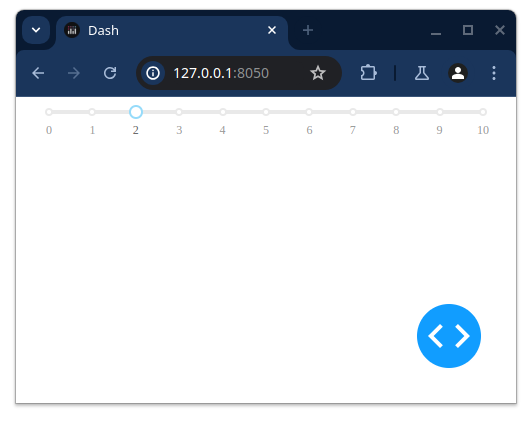
\includegraphics[width=5cm, height=5cm, keepaspectratio]{images/scatter_17.png}
				\end{center}
			\end{column}
		\end{columns}
	\end{frame}
	
	\begin{frame}[fragile]{Markerek testreszabása}
		\begin{columns}
			\begin{column}{.5\textwidth}
				A \texttt{marks} paraméter egy szótárat fogad, aminek a kulcsa a címke, és a hozzá tartozó érték egy másik szótár, amiben a címkéhez tartozó tulajdonságok vannak megadva.
				\begin{lstlisting}[language=python]
marks={
	0: {'label': '$1.9', 'style': {'color': cividis0, 'fontWeight': 'bold'}},
	1: {'label': '$3.2', 'style': {'color': cividis0, 'fontWeight': 'bold'}},
	2: {'label': '$5.5', 'style': {'color': cividis0, 'fontWeight': 'bold'}},
}				
				\end{lstlisting}
			\end{column}
			\begin{column}{.5\textwidth}
				\begin{center}
					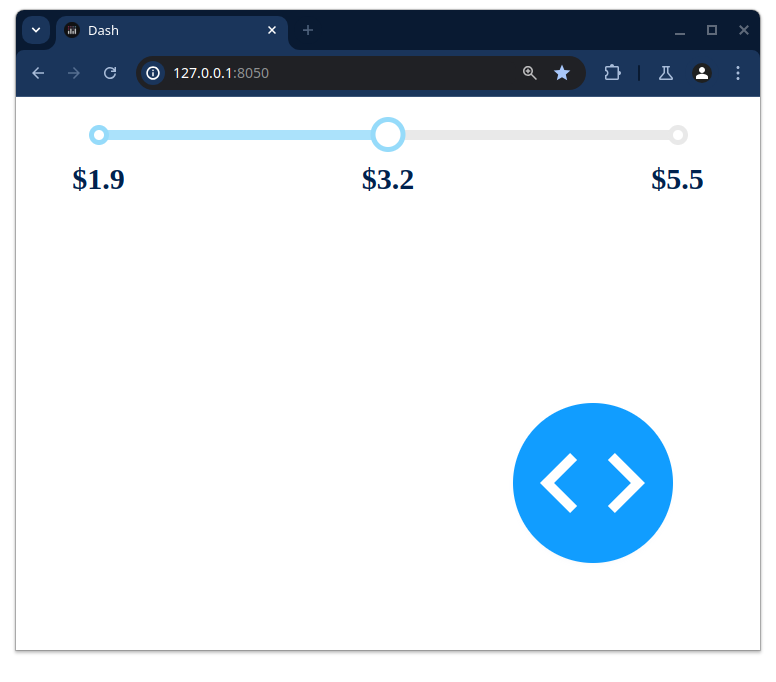
\includegraphics[width=5cm, height=5cm, keepaspectratio]{images/scatter_18.png}
				\end{center}
			\end{column}
		\end{columns}
	\end{frame}
	
	\begin{frame}{Alkalmazás csúszkákkal (\texttt{app\_v3\_1.py})}
		\begin{columns}
			\begin{column}{.5\textwidth}
				Az alkalmazás következő iterációjában két csúszka került hozzáadásra, az egyikkel a szegénységi szintet, a másikkal pedig az évet lehetséges kiválasztani.\par\medskip
				A hozzá tartozó callback függvény a csúszkák állapotának változásának hatására elindul, és leszűri a megfelelő adatkészletet. Az adatkészletből egy plotly diagramot állít elő és téríti vissza a megfelelő \texttt{Output} attribútumba.\par\medskip
				A teljes alkalmazásba való beépítést az \texttt{app\_v3\_2.py} valósítja meg.
			\end{column}
			\begin{column}{.5\textwidth}
				\begin{center}
					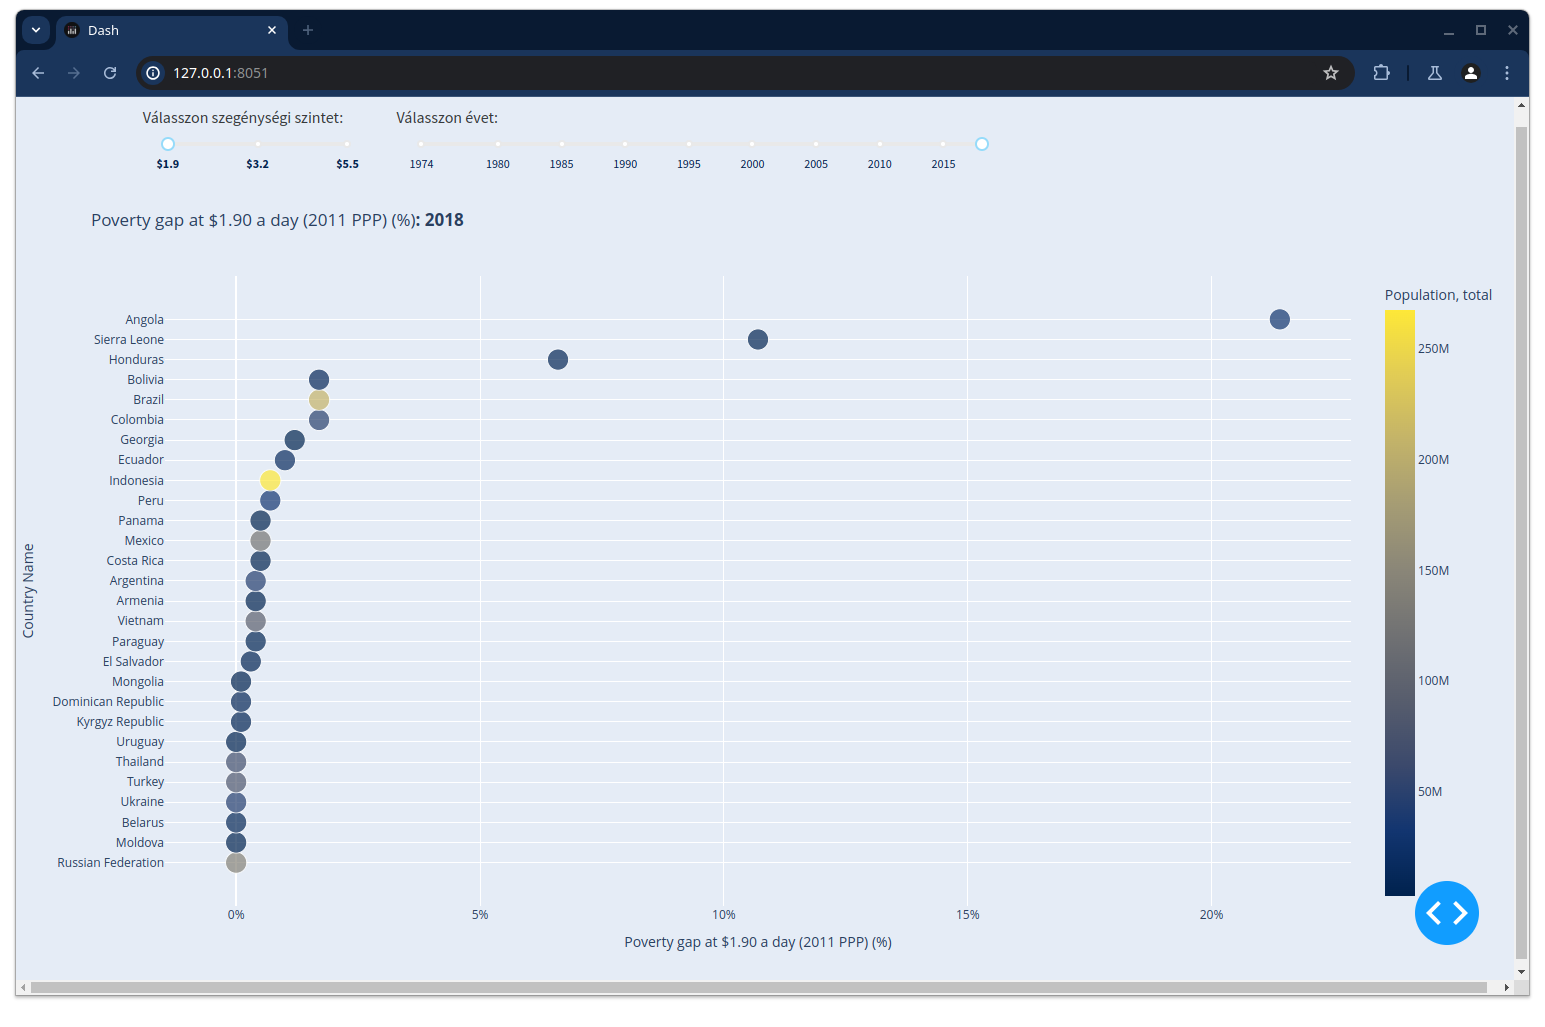
\includegraphics[width=7cm, height=5cm]{images/scatter_19.png}
				\end{center}		
			\end{column}
		\end{columns}
	\end{frame}
	
	\begin{frame}{Csúszkák beépítése az alkalmazásba (\texttt{app\_v3\_2.py})}
		\begin{center}
			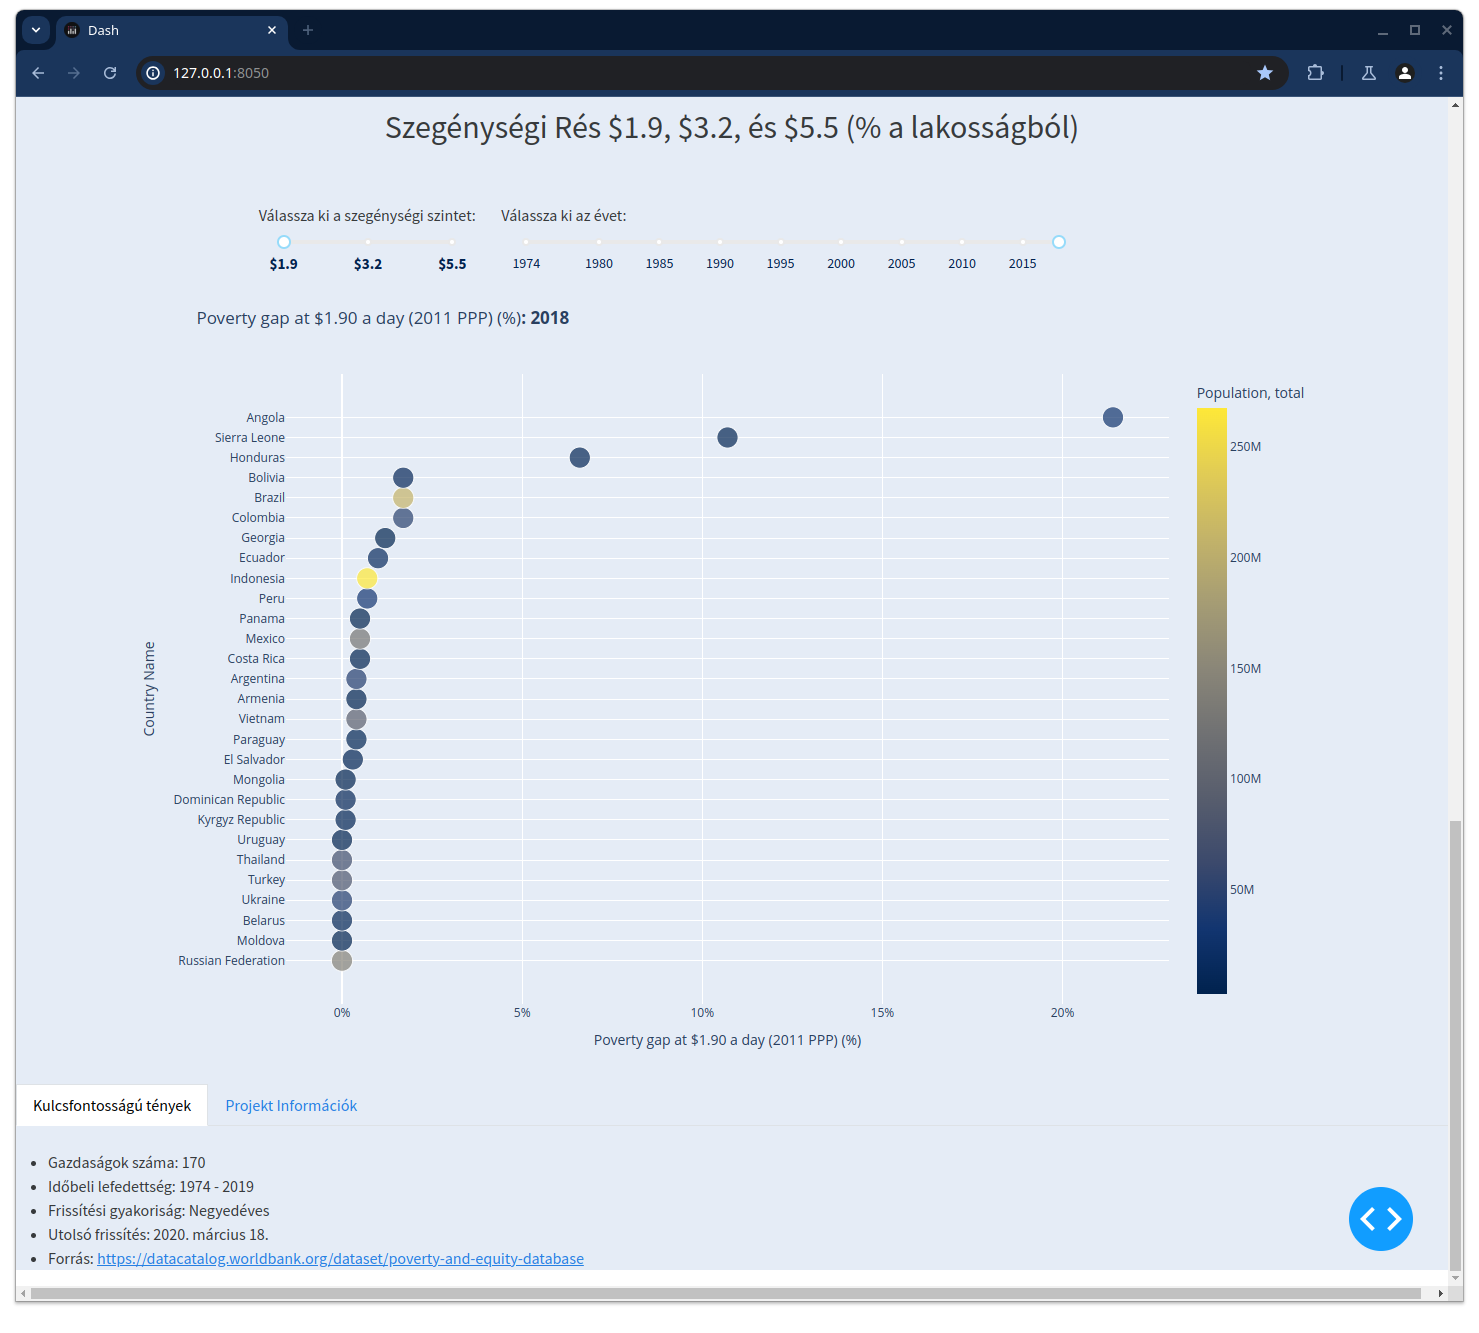
\includegraphics[width=7cm, height=7cm, keepaspectratio]{images/scatter_34.png}
		\end{center}
	\end{frame}
	
	\section{Tematikus térképek}
	
	\begin{frame}{}
		\tableofcontents[currentsection]
	\end{frame}
	
	\begin{frame}[fragile]{Egyszerű tematikus térkép}
		\begin{columns}
			\begin{column}{.5\textwidth}
				Egy tematikus térképhez szükség van egy érték oszlopra, és egy országkód oszlopra a rendelkezésre álló adatkészletben.\par\smallskip
				Az országkódokat általában ISO 3166-1 alpha-3 formátumban használja, ami hárombetűs kódokat jelent (pl. Magyarország esetében "HUN").\par\smallskip
				\begin{lstlisting}[language=python]
fig = px.choropleth(df, locations="Country Code", color=indicator)				
				\end{lstlisting}
			\end{column}
			\begin{column}{.5\textwidth}
				\begin{center}
					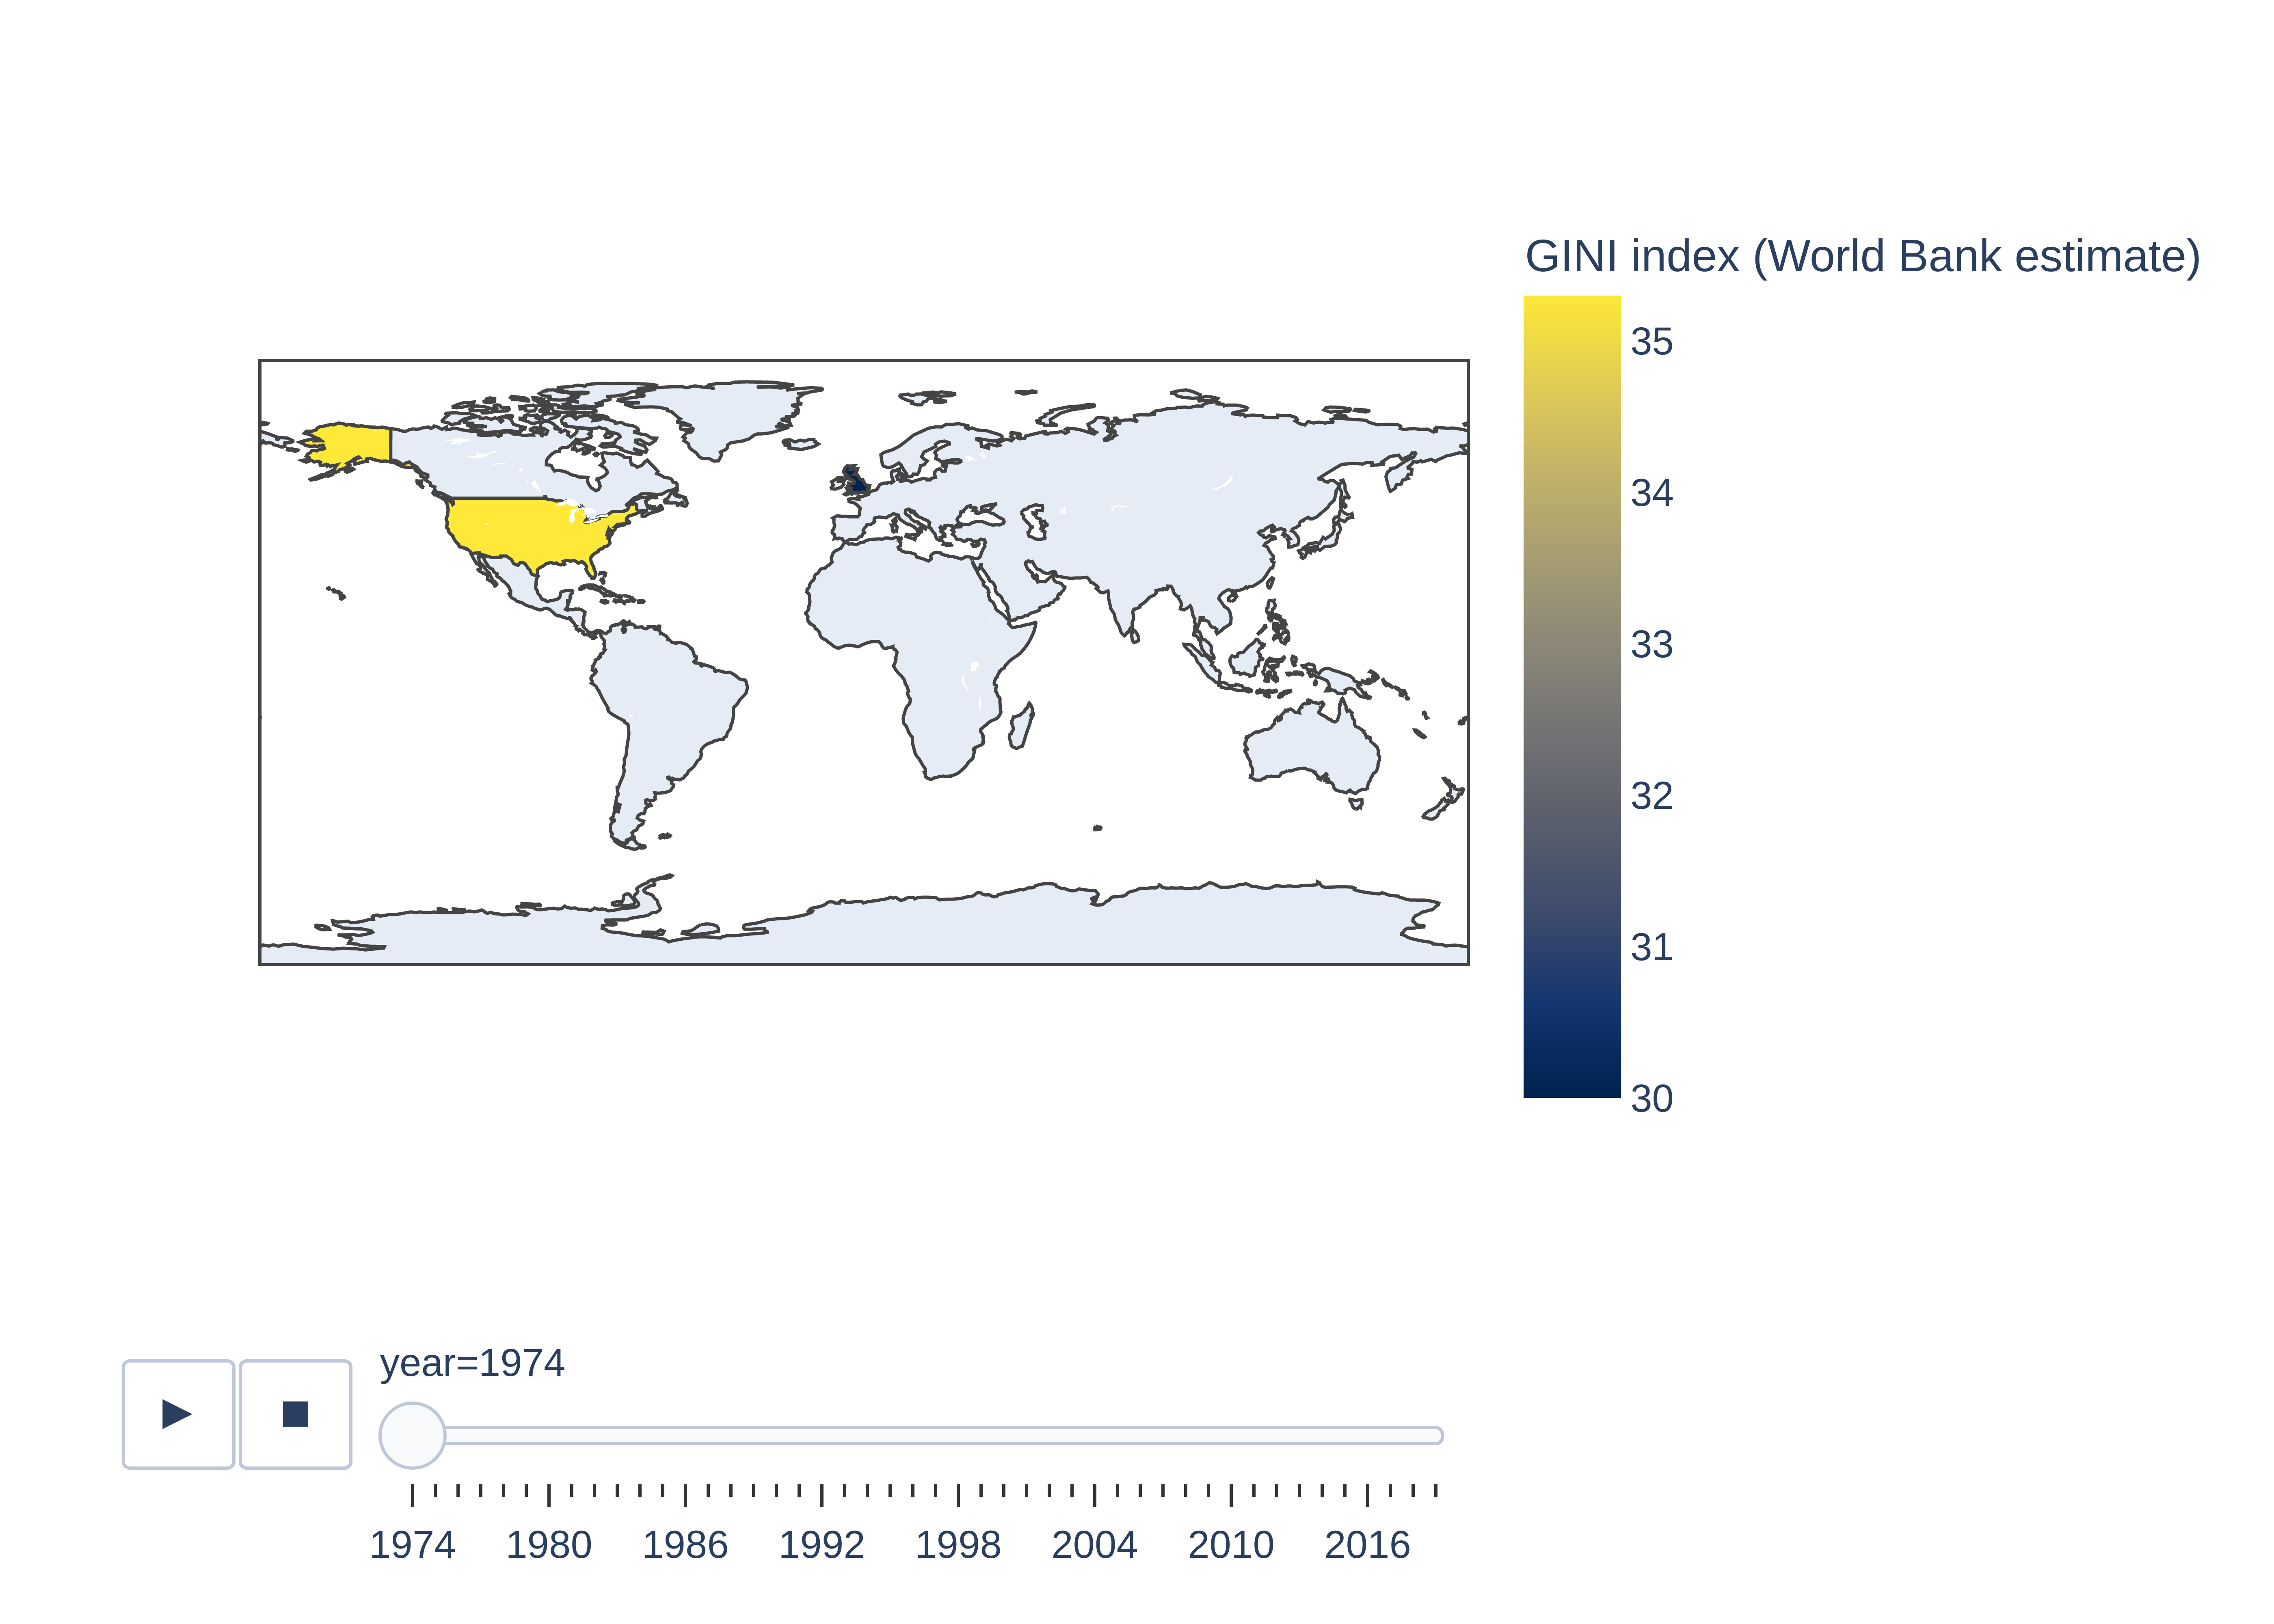
\includegraphics[width=7cm, height=7cm, keepaspectratio]{images/scatter_20.png}
				\end{center}
			\end{column}
		\end{columns}
	\end{frame}
	
	\begin{frame}[fragile]{Animációs réteg tematikus térképekkel}
		\begin{columns}
			\begin{column}{.5\textwidth}
				Az \texttt{animation\_frame} paraméterrel lehetséges bevezetni egy új, interaktív réteget adó komponenst, ami a választott változó alapján képes szekvenciálisan változtatni a megjelenített diagramot.\par\medskip
				\begin{lstlisting}[language=python]
fig = px.choropleth(
	poverty[poverty['is_country']],
	color_continuous_scale='cividis',
	locations='Country Code',
	color=indicator,
	animation_frame='year'
)				
				\end{lstlisting}
			\end{column}
			\begin{column}{.5\textwidth}
				\begin{center}
					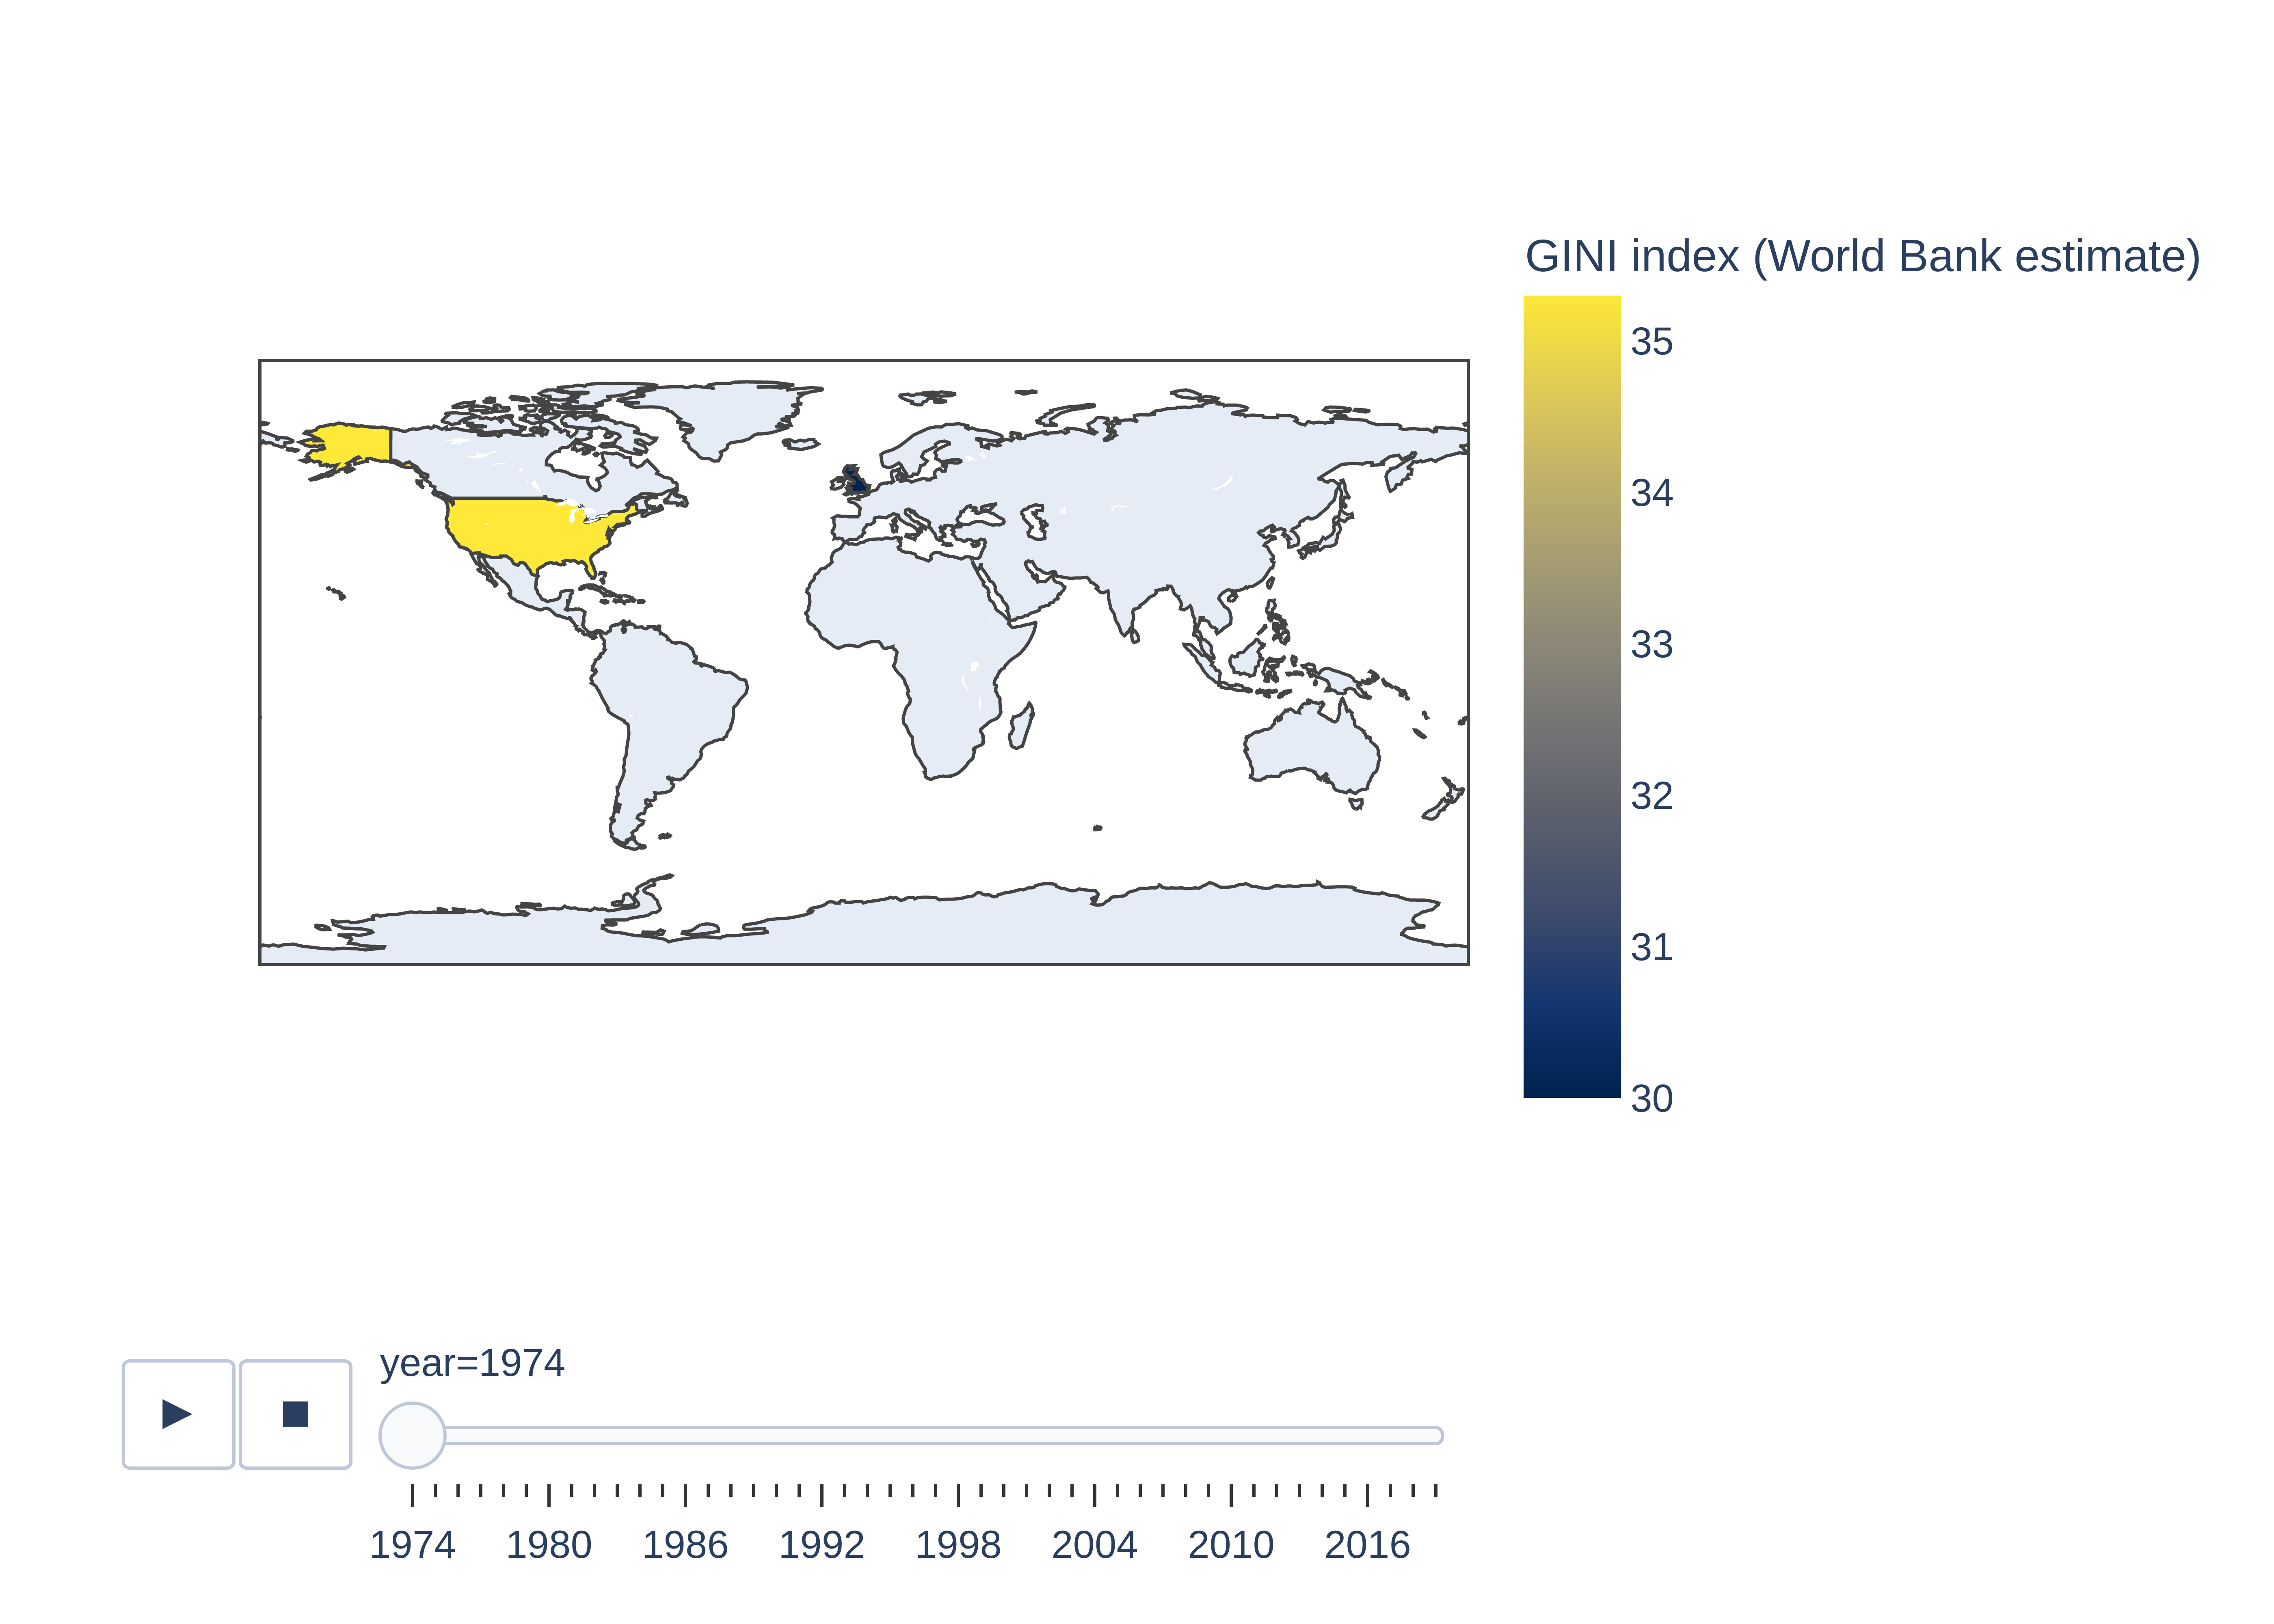
\includegraphics[width=7cm, height=7cm, keepaspectratio]{images/scatter_21.png}
				\end{center}
			\end{column}
		\end{columns}
	\end{frame}
	
	\begin{frame}{Fontosabb paraméterek tematikus térképekkel}
		\begin{columns}
			\begin{column}{.5\textwidth}
				\begin{itemize}
					\item \texttt{fig.layout.geo.showframe}: Eltünteti a keretet a térképdobozról
					\item \texttt{fig.layout.geo.showcountries}: Mutatja az országok keretezővonalait
					\item \texttt{fig.layout.geo.projection.type}: Térkép projekció állítása
					\item \texttt{fig.layout.geo.landcolor}: A föld színének állítása
					\item \texttt{fig.layout.geo.bgcolor}: Háttérszín a térképen
					\item \texttt{fig.layout.paper\_bgcolor}: Háttérszín a kereteződobozban
				\end{itemize}
			\end{column}
			\begin{column}{.5\textwidth}
				\begin{center}
					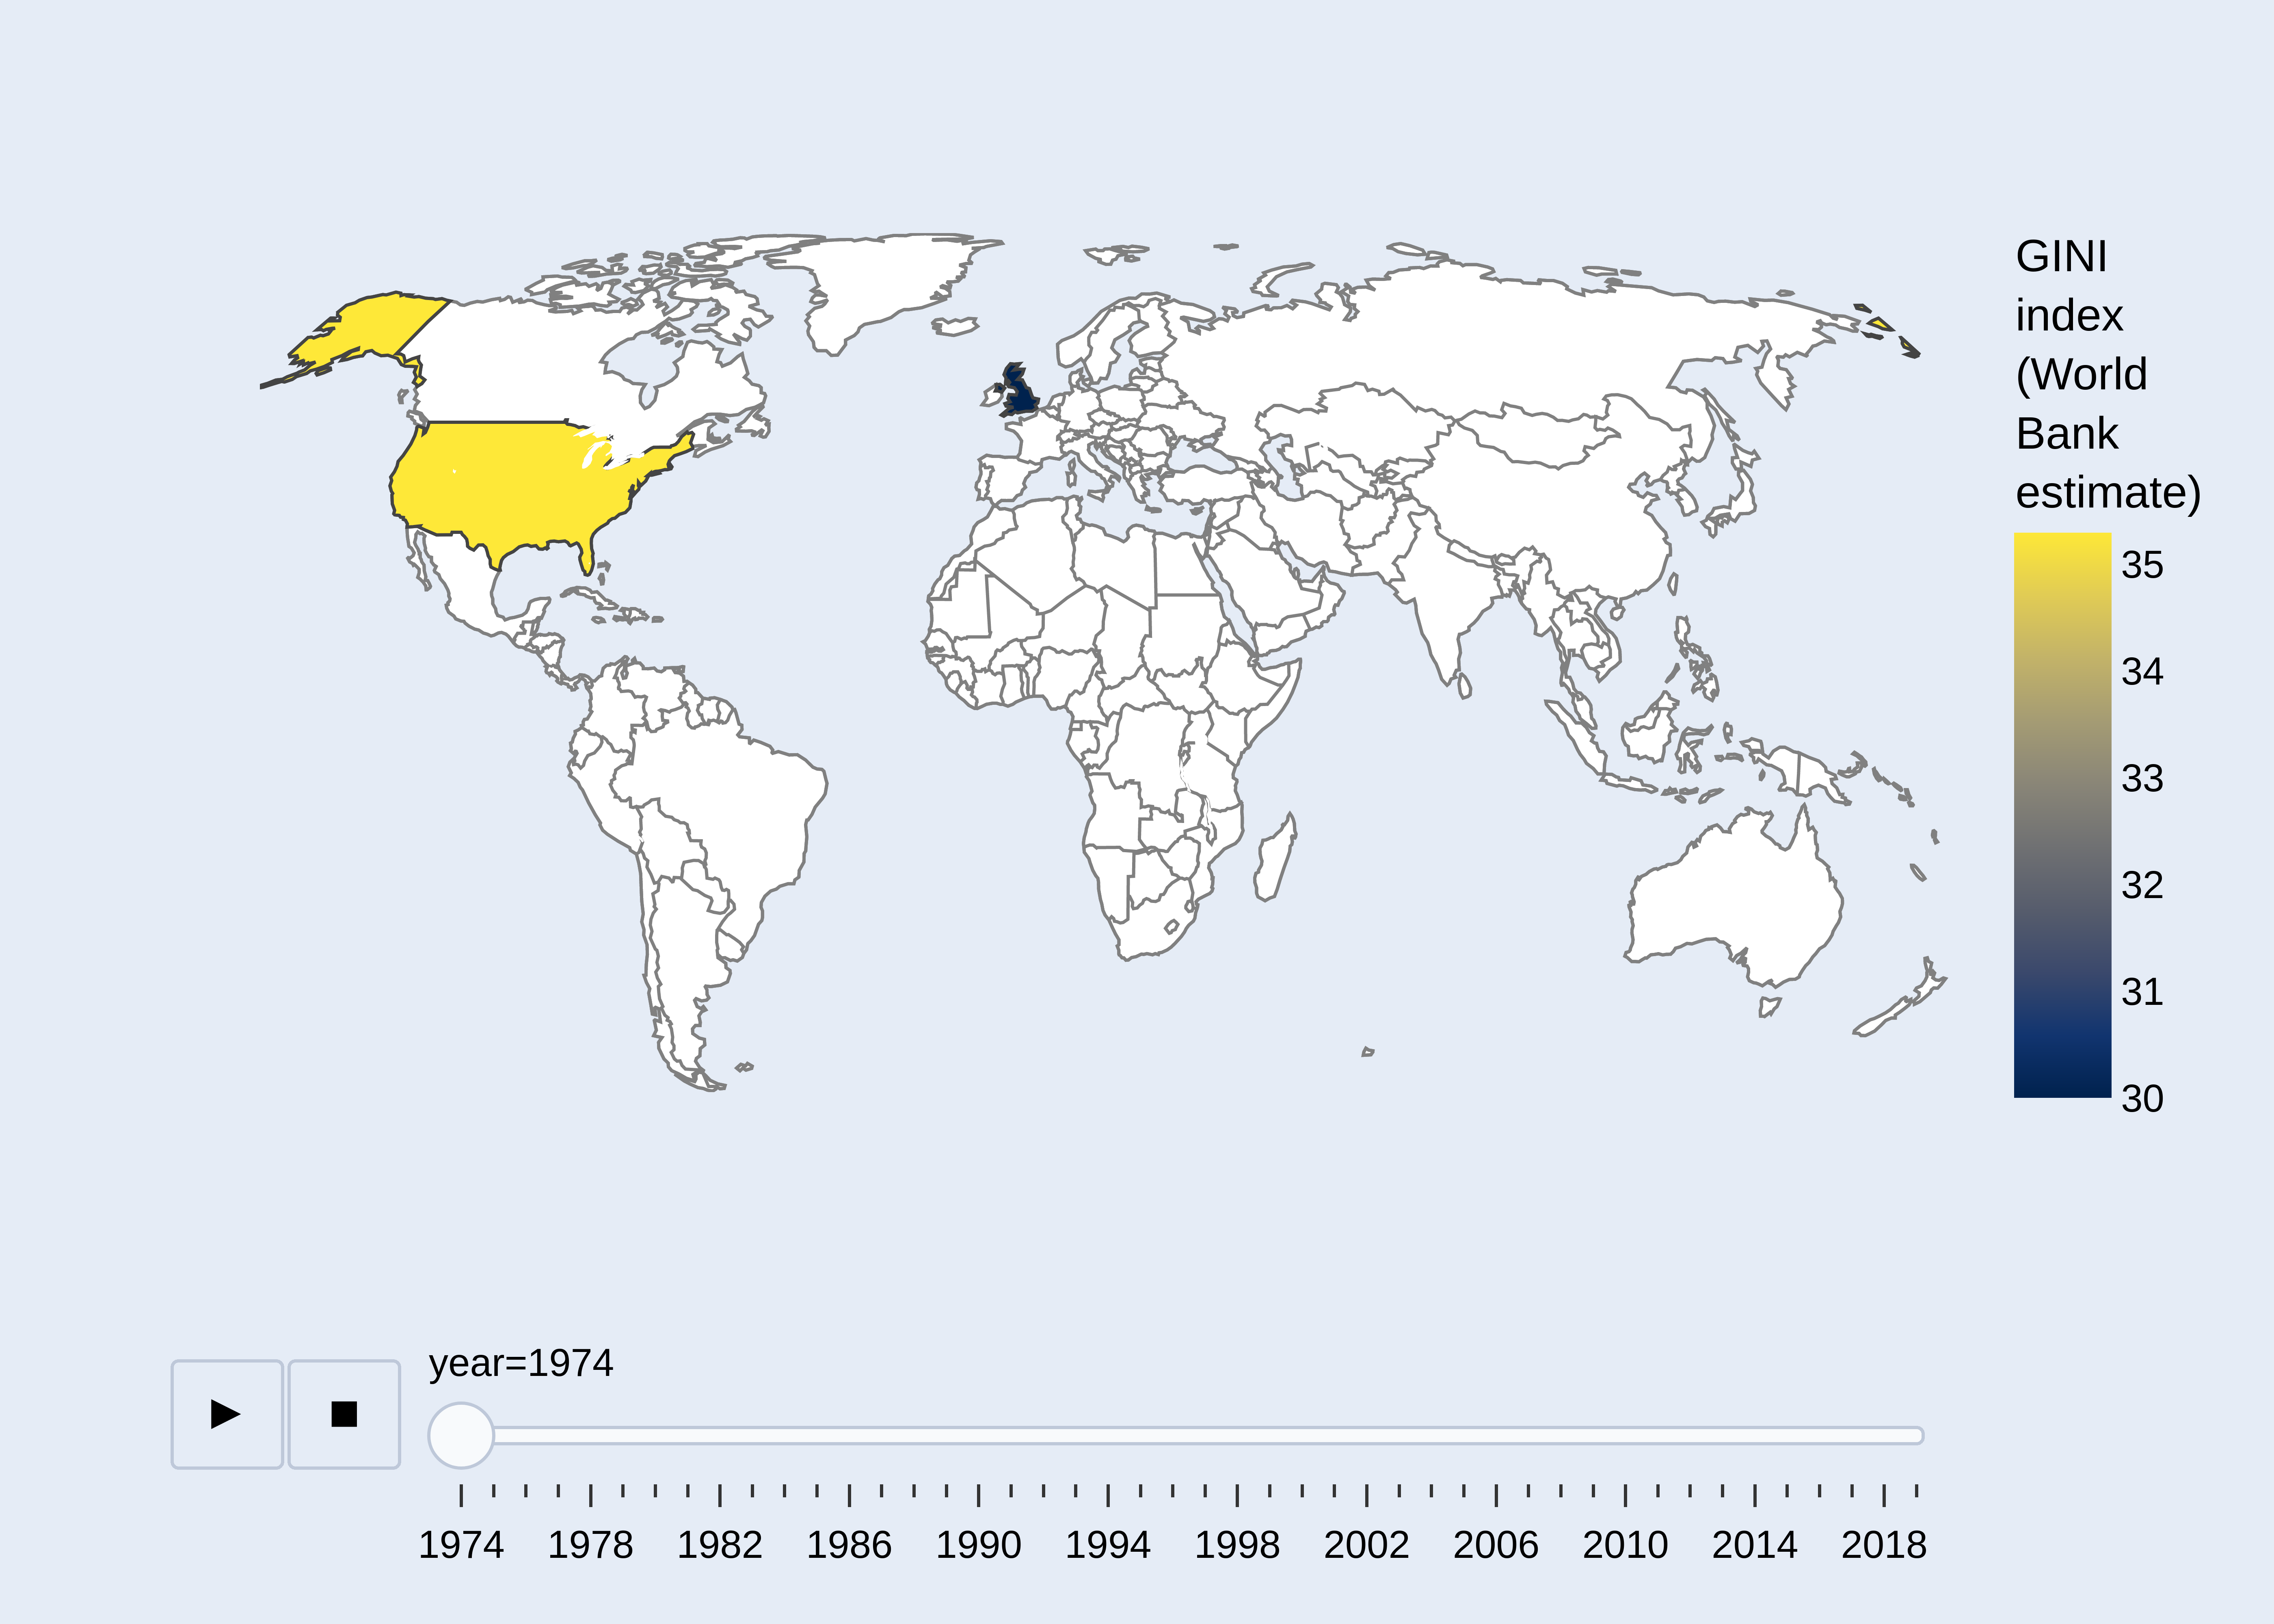
\includegraphics[width=7cm, height=7cm, keepaspectratio]{images/scatter_22.png}
				\end{center}
			\end{column}
		\end{columns}
	\end{frame}
	
	\begin{frame}[fragile]{Callback függvények térképekkel}
		\begin{columns}
			\begin{column}{.5\textwidth}
				\begin{enumerate}
					\item Új \texttt{DropDown} komponens létrehozása:
					\begin{lstlisting}[language=python]
	dcc.Dropdown(
		id='indicator_dropdown',
		value='GINI index (World Bank estimate)',
		options=[{'label': indicator, 'value': indicator} for indicator in poverty.columns[3:54]]
	)
					\end{lstlisting}
					\item \texttt{Graph} komponens létrehozása a térképnek: 
					\begin{lstlisting}[language=python]
	dcc.Graph(id='indicator_map_chart')
					\end{lstlisting}
				\end{enumerate}
			\end{column}
			\begin{column}{.5\textwidth}
				\begin{enumerate}
					\setcounter{enumi}{2}
					\item Callback függvény létrehozása
					\begin{lstlisting}[language=python]
@app.callback(
	Output('indicator_map_chart', 'figure'),
	Input('indicator_dropdown', 'value'))
def display_generic_map_chart(indicator):
	df = poverty[poverty['is_country']]
	fig = px.choropleth(
		df,
		locations='Country Code',
		color=indicator,
		...
	)
	fig.layout.geo.showframe = False
	...
	return fig
					\end{lstlisting}
				\end{enumerate}
			\end{column}
		\end{columns}
	\end{frame}
	
	\begin{frame}[fragile]{Alkalmazás legördülő menüvel és tematikus térképpel (\texttt{map\_app\_v1.py})}
		\begin{columns}
			\begin{column}{.5\textwidth}
				Az alkalmazás működésének megfelelően a felhasználó kiválaszthat egy indikátort a \texttt{Dropdown} menüből, ez elindít egy callback függvényt, aminek átadódik az indikátor értéke.\par\smallskip
				A legördülő menü állapotát felhasználva a callback függvény renderel egy tematikus térképet, és felülírja a \texttt{Graph} komponens \texttt{figure} attribútumát.
			\end{column}
			\begin{column}{.5\textwidth}
				\begin{center}
					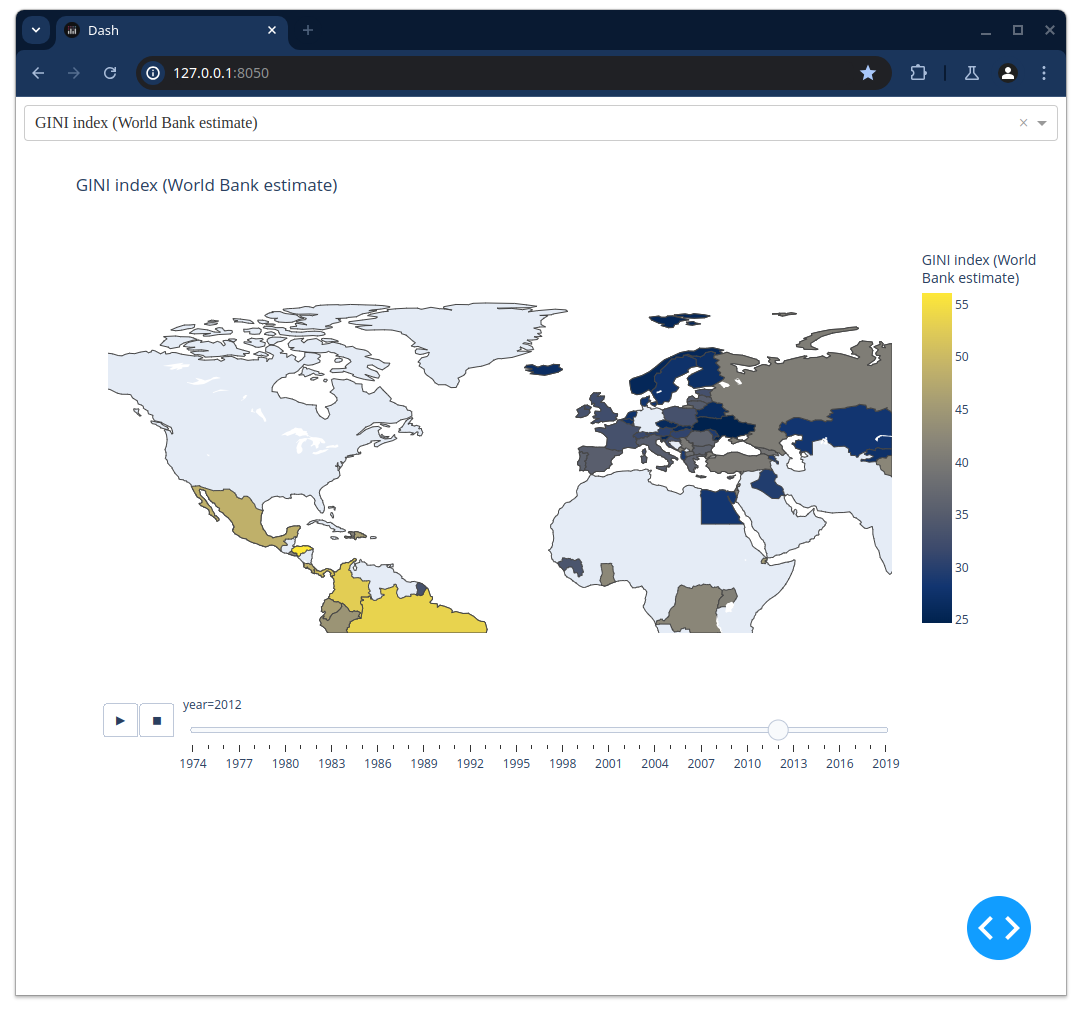
\includegraphics[width=7cm, height=7cm, keepaspectratio]{images/scatter_23.png}
				\end{center}
			\end{column}
		\end{columns}
	\end{frame}
	
	\begin{frame}[fragile]{\texttt{dcc.Store} komponensek}
		\begin{columns}
			\begin{column}{.5\textwidth}
				\only<1>{
					A tároló komponenseket arra lehet használni, hogy a kliens oldalon tároljon el adatot anélkül, hogy azt visszaküldené a szervernek.\par\smallskip
					Dash alkalmazásokban a \texttt{dcc.Store} komponensek tartalmát callback függvények segítségével lehet manipulálni.
				}
				\only<2>{
					A \texttt{Store} komponenseknek 3 típusa létezik:
					\begin{itemize}
						\item \texttt{memory}: Az adat a böngésző memóriájában tárolódik, és törlődik, amikor az oldalt frissíti a felhasználó
						\item \texttt{local}: Az adat a böngésző helyi tárhelyén tárolódik el, és frissítés után nem törlődik
						\item \texttt{session}: Az adat a böngésző munkamenete során marad meg, és akkor törlődik, amikor a felhasználó bezárja a megfelelő lapot
					\end{itemize}
				}
			\end{column}
			\begin{column}{.5\textwidth}
				\begin{lstlisting}[language=python]
app.layout = html.Div([
	dcc.Store(id='store', storage_type='session'),
])	

@app.callback(
	Output('my-store', 'data'),
	Input('save-button', 'n_clicks')
)
def save_data(n_clicks):
if n_clicks:
	return {'key': 'value'}
return dash.no_update							
				\end{lstlisting}
			\end{column}
		\end{columns}
	\end{frame}
	
	\begin{frame}[fragile]{\texttt{dcc.Interval} komponensek}
		\begin{columns}
			\begin{column}{.5\textwidth}
				A \texttt{dcc.Interval} komponenseket arra lehet használni, hogy egy adott callback függvényt elindítson az alkalmazás adott időközönként. Ilyen például adatkészletek, diagramok frissítése, vagy folyamatok állapotának ellenőrzése. Fontosabb paraméterei:
				\begin{itemize}
					\item \texttt{interval}: Az intervallum (ms) hossza, ami két callback indítás között eltelik
					\item \texttt{n\_intervals}: Az eltelt intervallumok számát tartalmazó attribútum
					\item \texttt{disabled}: Ha értéke \texttt{True}, a callback függvény nem indul el
				\end{itemize}
			\end{column}
			\begin{column}{.5\textwidth}
				\begin{lstlisting}[language=python]
app.layout = html.Div([
	dcc.Interval(
		id='interval-component', 
		interval=1 * 1000,
		n_intervals=0,
	),
])

@app.callback(
	Output('output', 'children'),
	Input('interval-component', 'n_intervals')
)
def update_output(n):
	return f'Interval has triggered {n} times.'				
				\end{lstlisting}
			\end{column}
		\end{columns}
	\end{frame}
	
	\begin{frame}{Alkalmazás \texttt{Storage} és \texttt{Interval} komponensekkel (\texttt{map\_app\_v2.py})}
		\begin{columns}
			\begin{column}{.6\textwidth}
				\texttt{dcc.Storage}:
				\begin{itemize}
					\item A \texttt{store\_data} callback frissíti a \texttt{dcc.Store} komponens \texttt{data} attribútumát a Világbank adataival minden alkalommal, amikor a \texttt{dcc.Interval} komponens frissítést indít.
				\end{itemize}
				\texttt{dcc.Interval}:
				\begin{itemize}
					\item A \texttt{store\_data} callback minden alkalommal aktiválódik, amikor a \texttt{dcc.Interval} komponens növeli az \texttt{n\_intervals} attribútum értékét. Ez biztosítja, hogy a Világbank adatai minden percben frissüljenek és tárolódjanak a \texttt{dcc.Store} komponensben.
				\end{itemize}
			\end{column}
			\begin{column}{.4\textwidth}
				\begin{center}
					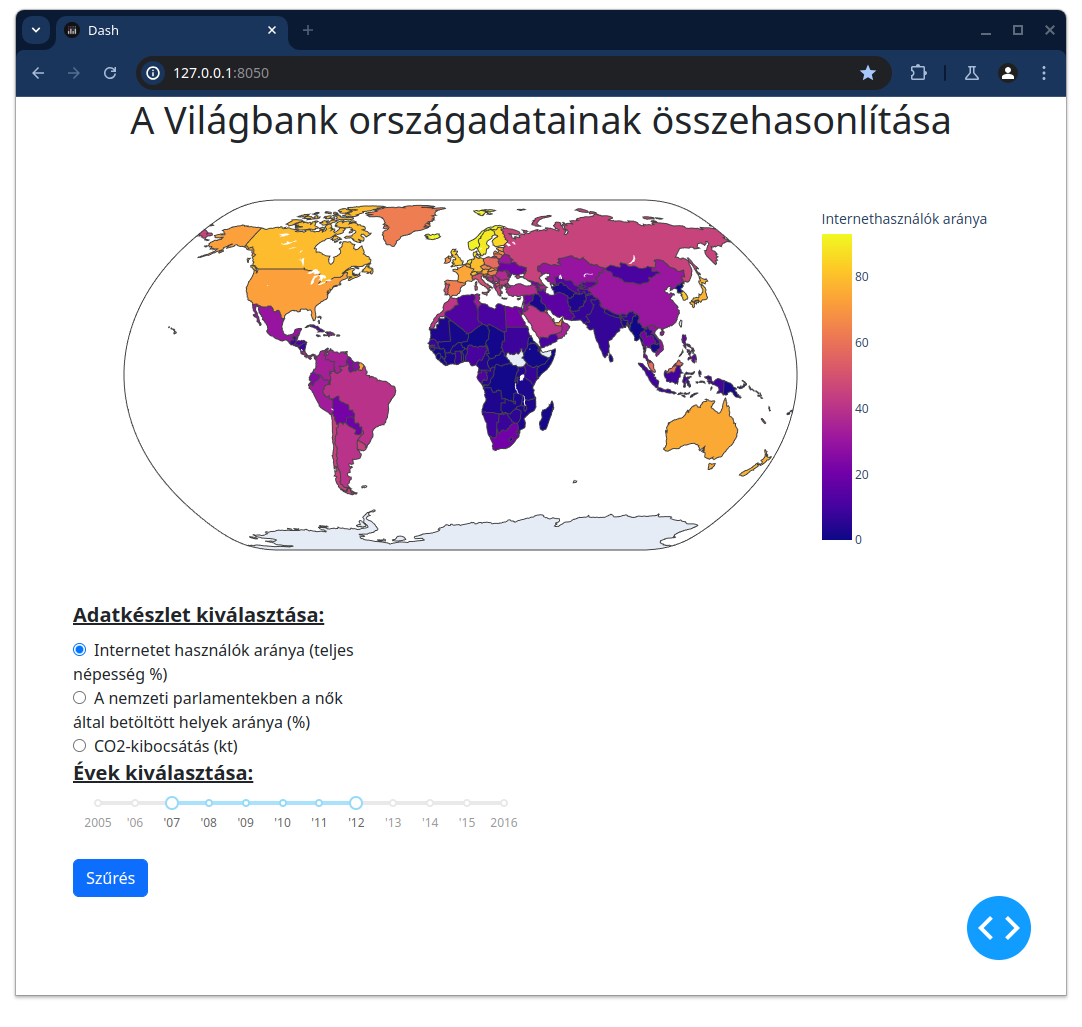
\includegraphics[width=6cm, height=6cm, keepaspectratio]{images/scatter_24.png}
				\end{center}
			\end{column}
		\end{columns}
	\end{frame}
	
	\section{Pontdiagramok térképekkel}
	
	\begin{frame}{}
		\tableofcontents[currentsection]
	\end{frame}
	
	\begin{frame}{Térkép projekciók}
		\begin{columns}
			\begin{column}{.5\textwidth}
				\only<1>{
					A térkép projekció egy matematikai módszer melynek feladata, hogy a Föld gömbölyű felületét egy síkra vetítse.\par\smallskip
					A folyamat során szükségszerűen torzulások keletkeznek.				
				}
				\only<2-4>{
					\begin{itemize}
						\item \textbf{Equirectangular}: A legegyszerűbb projekció, ahol a földrajzi szélesség és hosszúság egyenesen arányosan van ábrázolva a síkon.
						\item \textbf{Mercator}: Szögtartó, tehát a szögek és az irányok helyesek maradnak, így hasznos a navigációban.
						\item \textbf{Orthographic}: Háromdimenziós gömböt ábrázol síkban úgy, mintha egy távoli pontból néznénk.
						\item \textbf{Sinusoidal}: Ez az egyenlő területű projekció, amely megőrzi a területek arányait.
					\end{itemize}
				}
			\end{column}
			\begin{column}{.5\textwidth}
				\begin{center}
					\includegraphics<1>[width=7cm, height=7cm, keepaspectratio]{images/scatter_25}
					\includegraphics<2>[width=7cm, height=7cm, keepaspectratio]{images/scatter_26}
					\includegraphics<3>[width=7cm, height=7cm, keepaspectratio]{images/scatter_27}
					\includegraphics<4>[width=7cm, height=7cm, keepaspectratio]{images/scatter_28}
				\end{center}
			\end{column}
		\end{columns}
	\end{frame}
	
	\begin{frame}[fragile]{Pontdiagramok térképekkel}
		\begin{columns}
			\begin{column}{.5\textwidth}
				A plotly könyvtár alapértelmezetten támogatja az ISO-alpha3 országkódok pontos pozíciójának ábrázolását, ezért amikor paraméterül megkapja a \texttt{locations='Country Code'} értéket innen ki tudja olvasni az adott ország hosszúsági és szélességi koordinátáit.\par\smallskip
				\begin{lstlisting}[language=python]
df = poverty[poverty['year'].eq(2010) & poverty['is_country']]
fig = px.scatter_geo(df, locations='Country Code')				
				\end{lstlisting}
			\end{column}
			\begin{column}{.5\textwidth}
				\begin{center}
					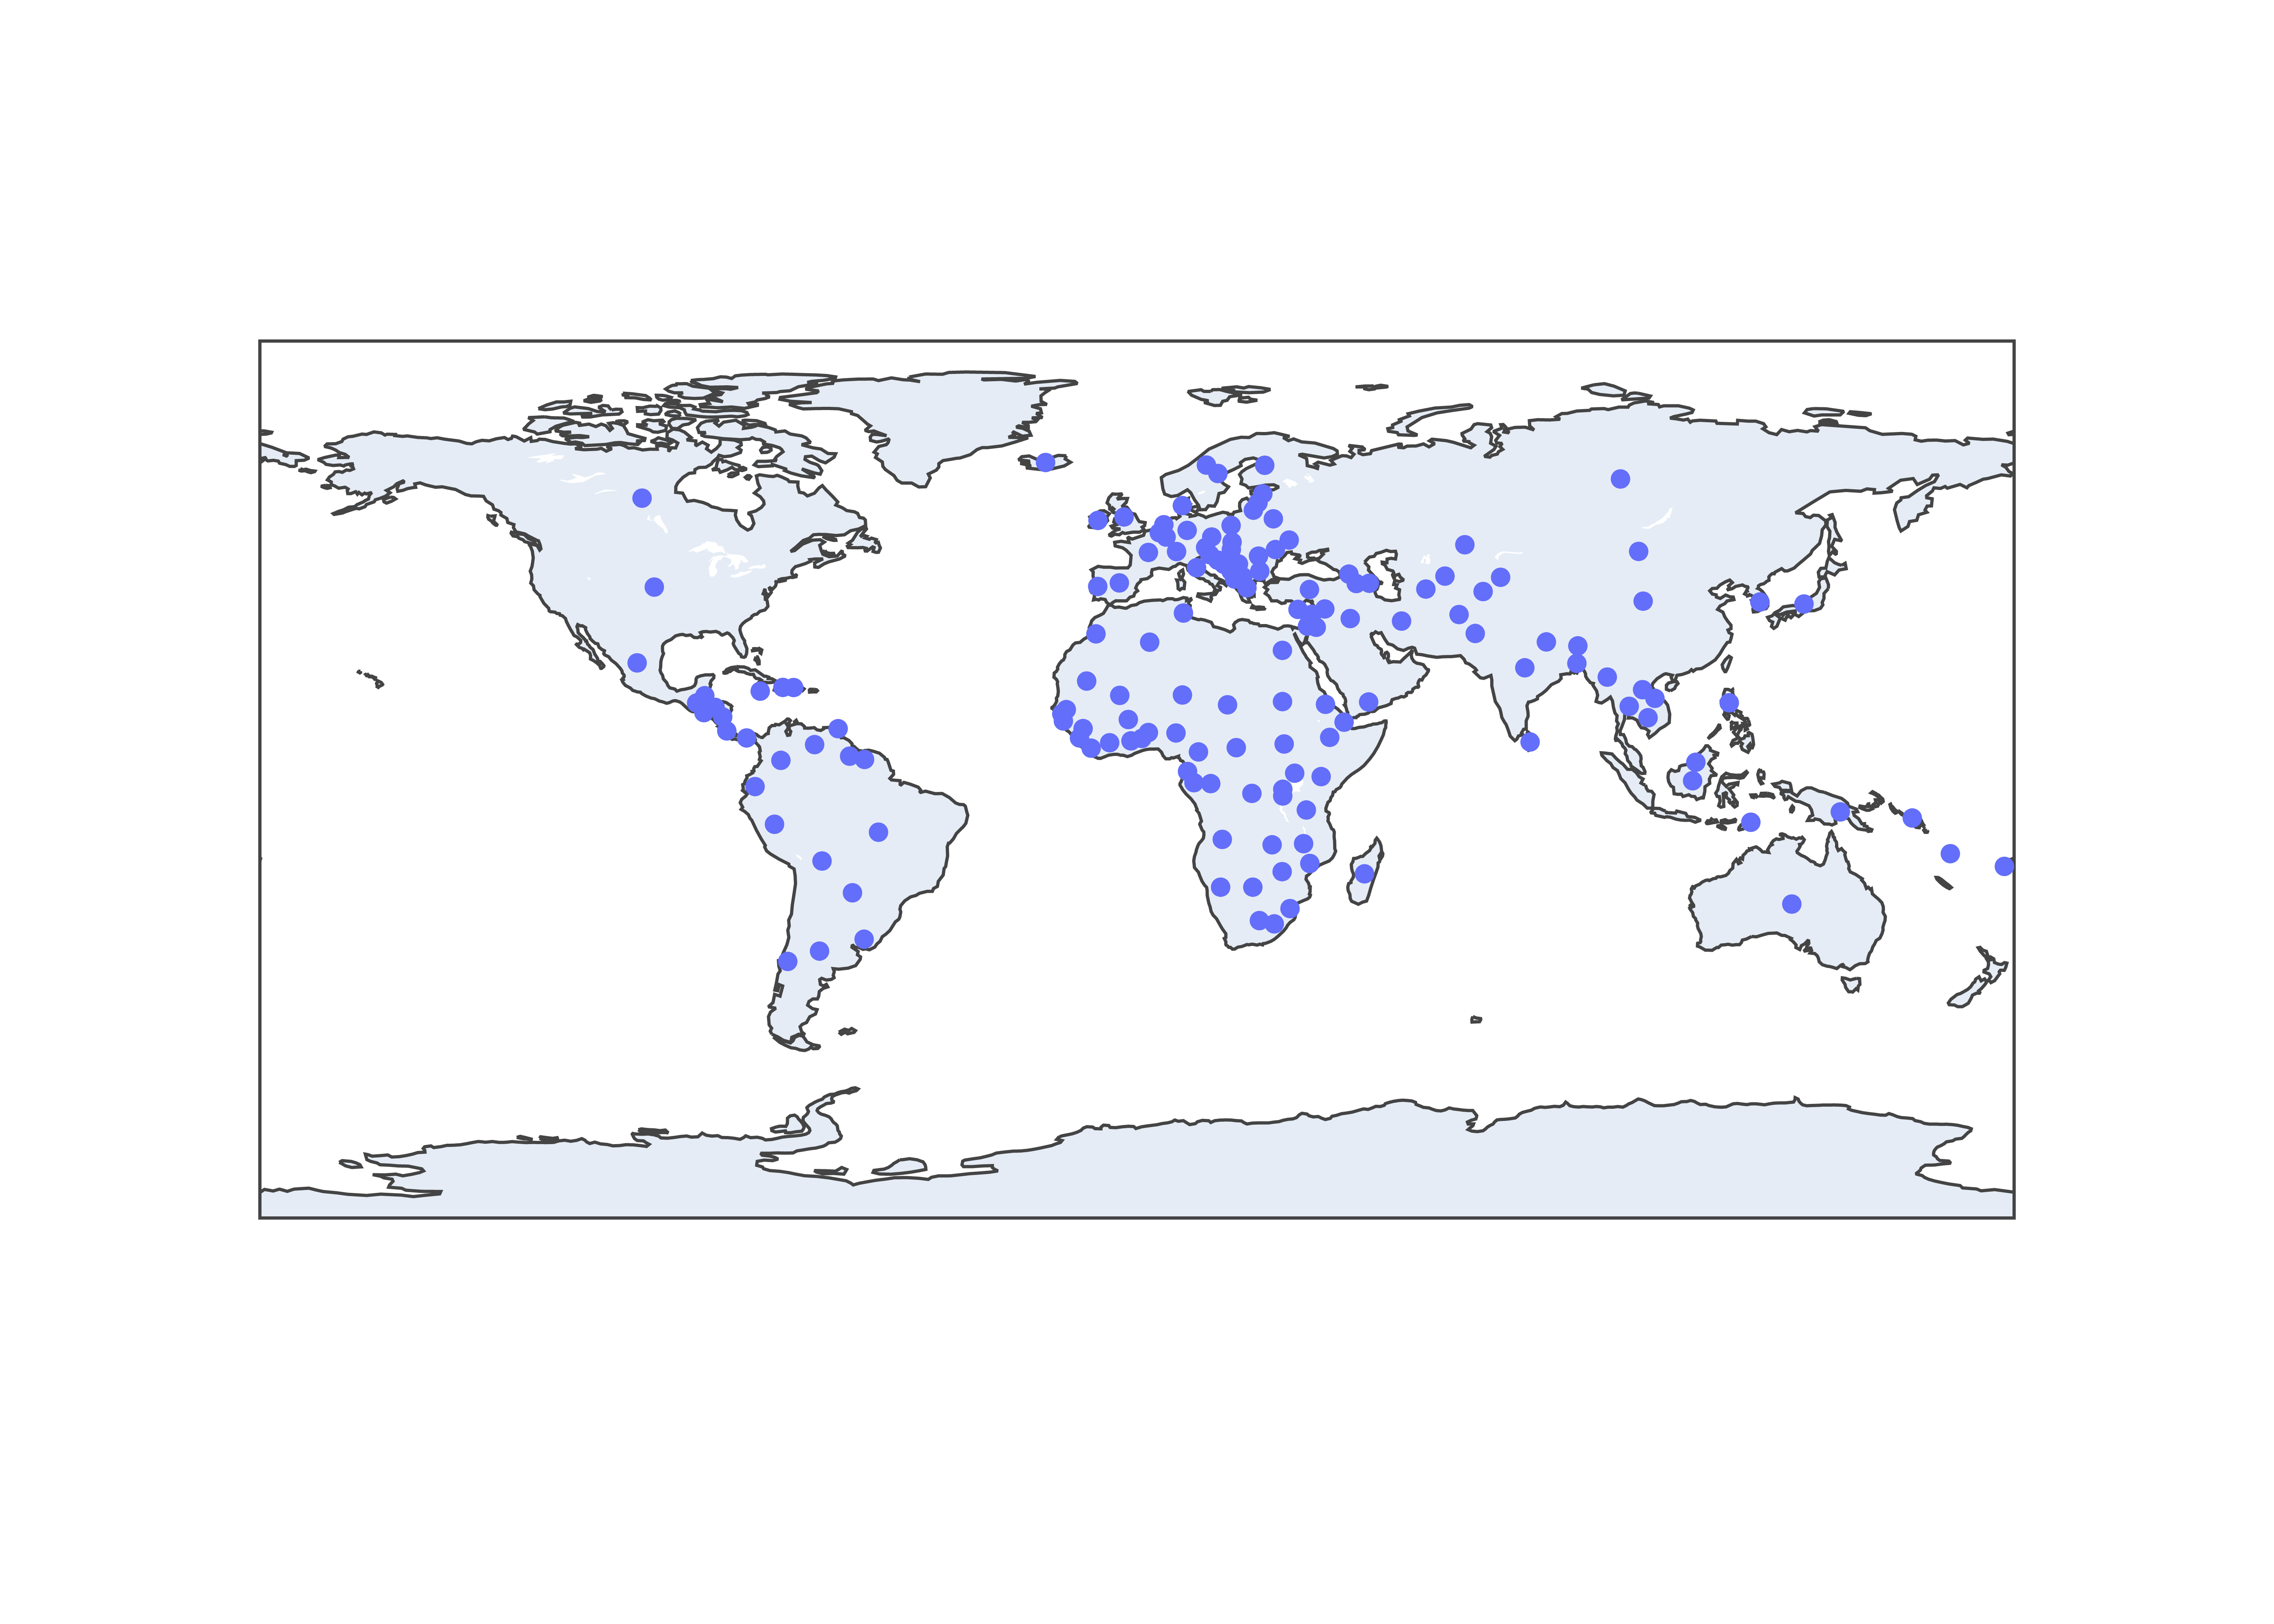
\includegraphics[width=7cm, height=7cm, keepaspectratio]{images/scatter_29.png}
				\end{center}
			\end{column}
		\end{columns}
	\end{frame}
	
	\begin{frame}[fragile]{\texttt{Mapbox} térképek}
		\begin{columns}
			\begin{column}{.5\textwidth}
				A \texttt{zoom} paraméter állításával lehetséges ráközelíteni a diagramra, a \texttt{center} paraméter a közelítés központját adja meg, és a \texttt{mapbox\_style} pedig a térképstílust.\par\medskip
				\begin{lstlisting}[language=python]
px.scatter_mapbox(
	lon=[5, 10, 15, 20],
	lat=[10, 7, 18, 5],
	zoom=2,
	center={'lon': 5, 'lat': 10},
	size=[5]*4,
	color_discrete_sequence=['darkred'],
	mapbox_style='stamen-watercolor'
)				
				\end{lstlisting}
			\end{column}
			\begin{column}{.5\textwidth}
				\begin{center}
					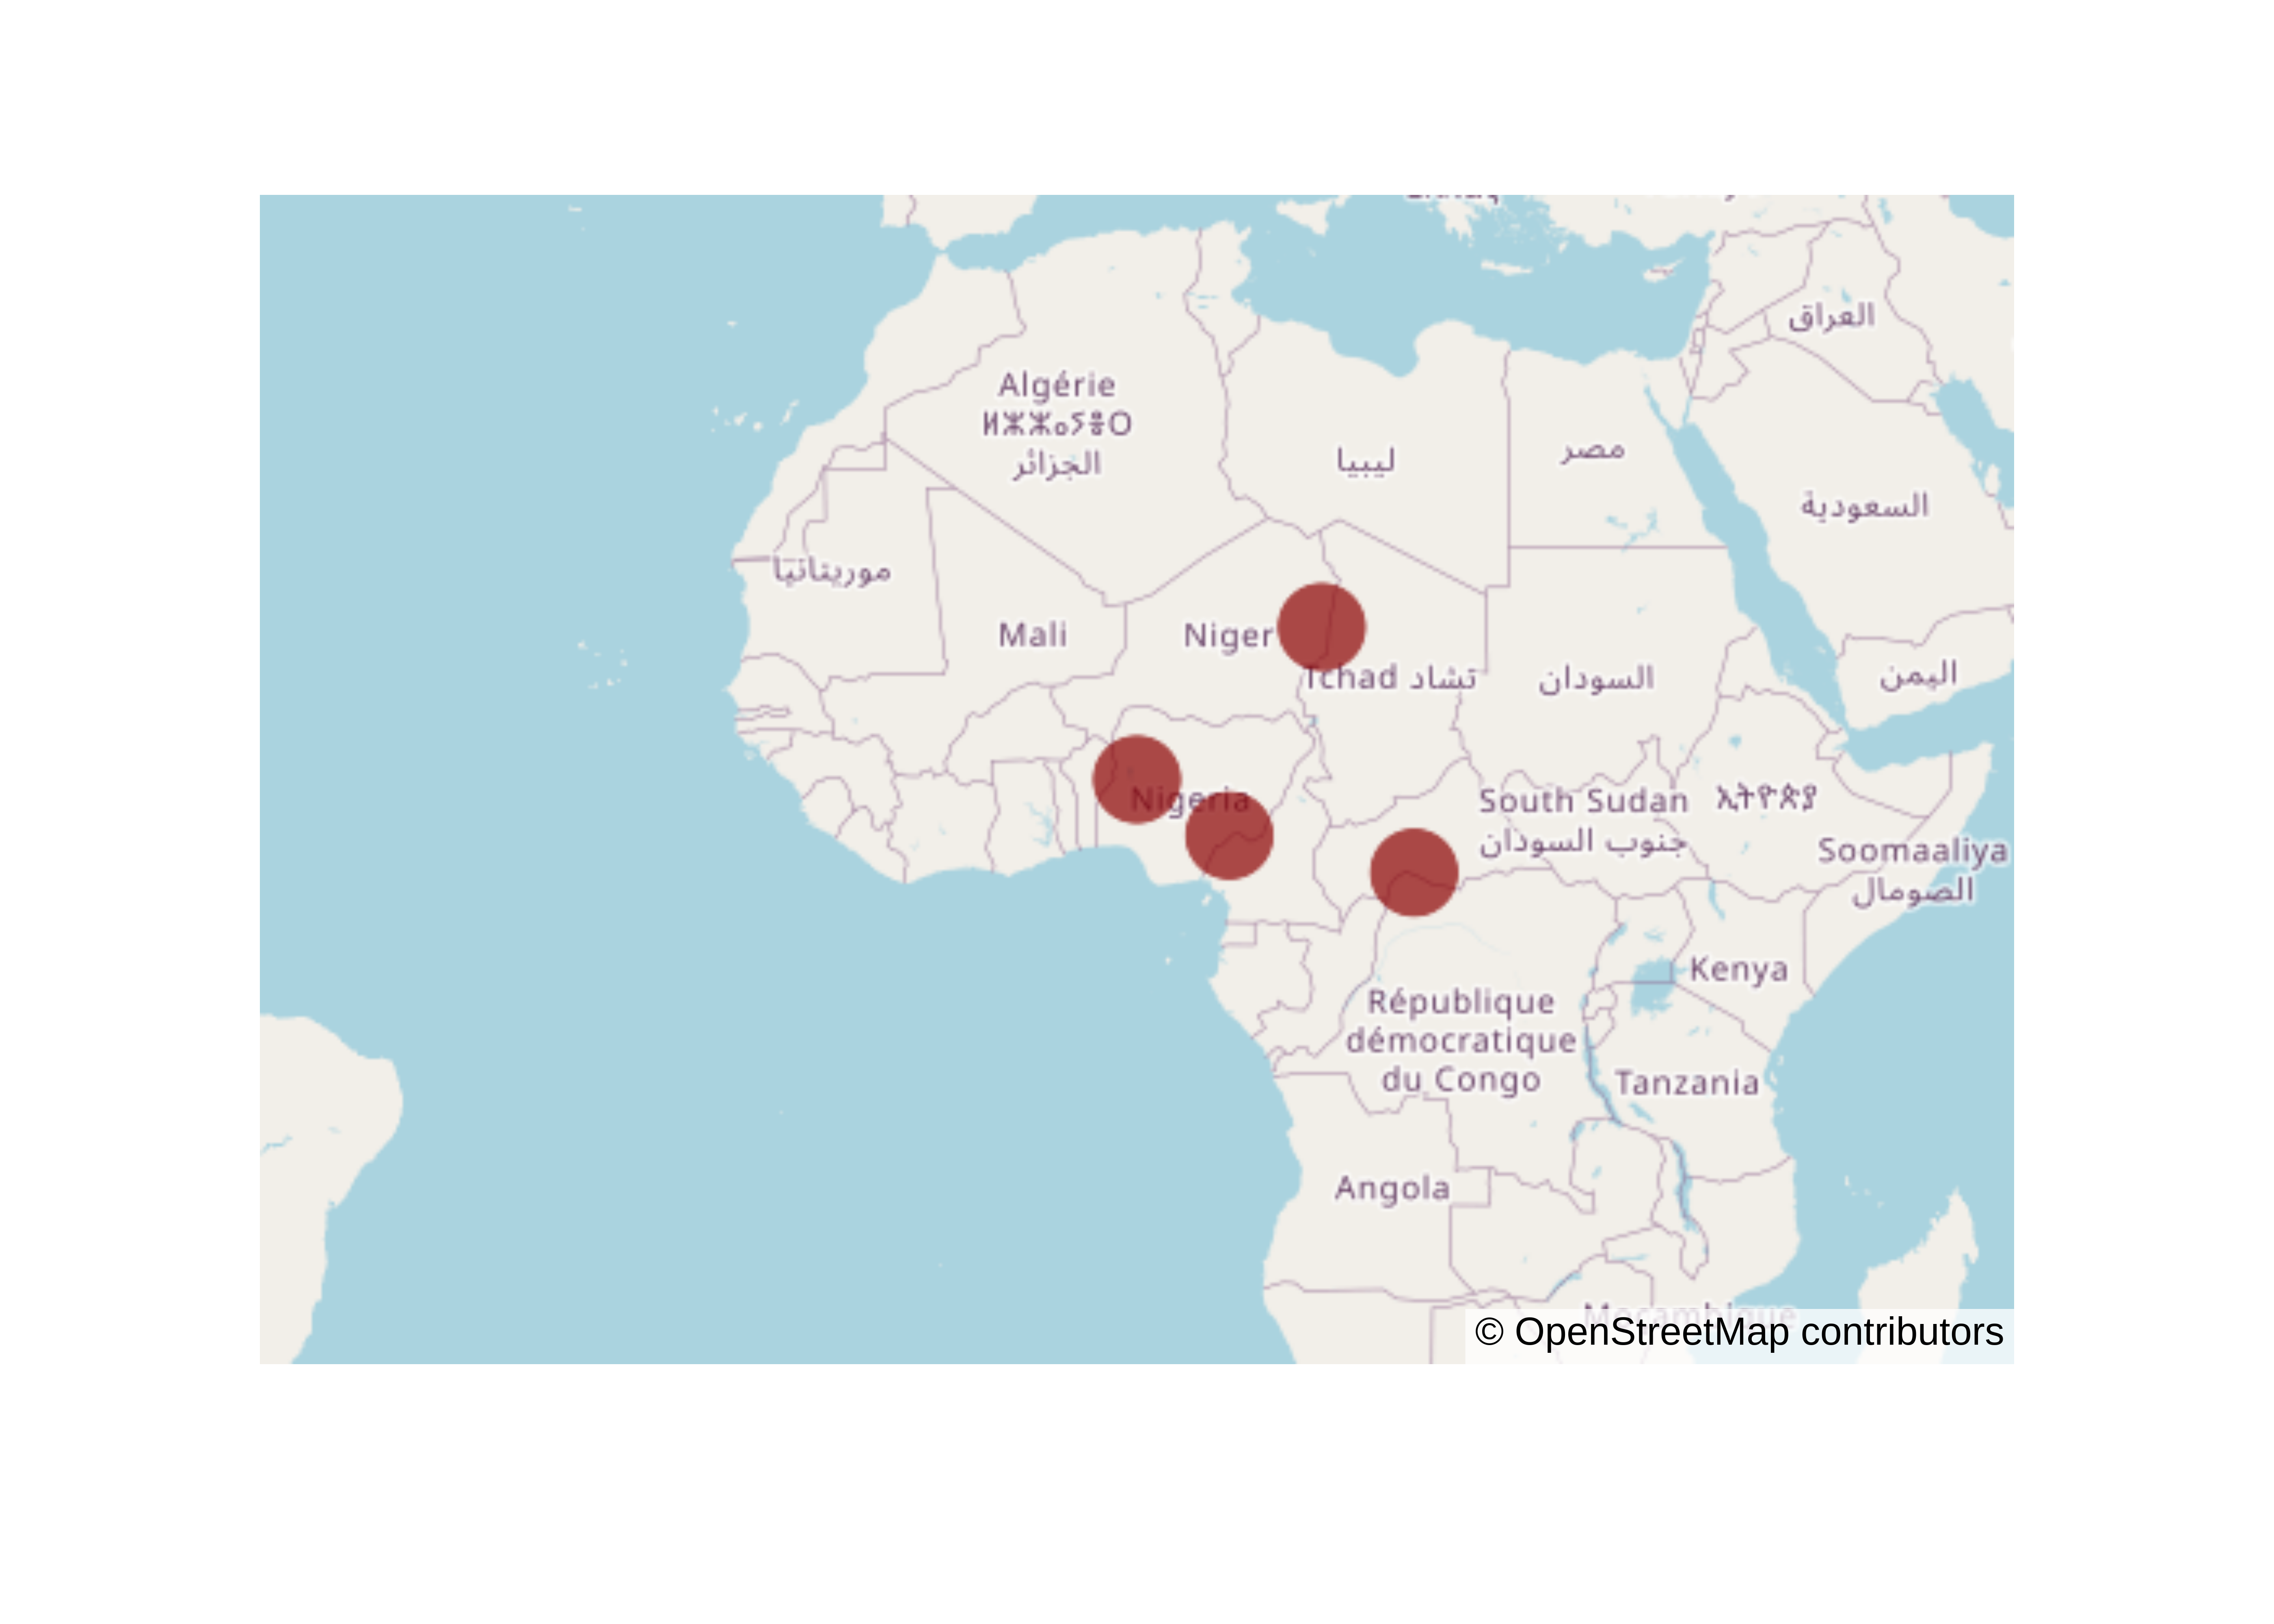
\includegraphics[width=7cm, height=7cm, keepaspectratio]{images/scatter_30.png}
				\end{center}
			\end{column}
		\end{columns}
	\end{frame}
	
	\section{Markdown}
	
	\begin{frame}{}
		\tableofcontents[currentsection]
	\end{frame}
	
	\lstset{
		basicstyle=\color{black}\ttfamily\scriptsize,
		keywordstyle=\color{black},
		commentstyle=\color{black},	
		stringstyle=\color{black},
		identifierstyle=\color{black},
		numberstyle=\color{black},	
	}
	
	\begin{frame}[fragile]{Markdown alapjai}
		A Markdown nyelv segítségével egyszerűen lehet HTML struktúrát létrehozni. Az outputot úgy jeleníti meg, mint bármelyik HTML dokumentum, de a megírása sokkal egyszerűbb.
		\begin{columns}
			\begin{column}{.5\textwidth}
				\begin{block}{HTML}
					\begin{center}
						\begin{minipage}{.8\textwidth}
							\begin{lstlisting}[language=bash]
<h1>Főcím</h1>
<h2>Alcím</h2>
<ul>
	<li>Első elem</li>
	<li>Második elem</li>
	<li>Harmadik elem</li>
</ul>					
							\end{lstlisting}	
						\end{minipage}
					\end{center}
				\end{block}
			\end{column}
			\begin{column}{.5\textwidth}
				\begin{block}{Markdown}
					\begin{center}
						\begin{minipage}{.8\textwidth}
							\begin{lstlisting}
# Főcím
## Alcím
* Első elem
* Második elem
* Harmadik elem
							\end{lstlisting}
						\end{minipage}
					\end{center}
				\end{block}			
			\end{column}
		\end{columns}
	\end{frame}
	
	\begin{frame}[fragile]{Markdown szabályai}
		\begin{columns}
			\begin{column}{.5\textwidth}
				\begin{itemize}
					\item Főcímek:
					\begin{lstlisting}[language=python]
# Első főcím
## Második főcím
### Harmadik főcím
					\end{lstlisting}
					\item Formázások:
					\begin{lstlisting}[language=python]
*Dőlt*
**Félkövér**
***Félkövér és dőlt***
					\end{lstlisting}
					\item Linkek:
					\begin{lstlisting}[language=python]
[Link szöveg](URL)
					\end{lstlisting}
					\item Képek:
					\begin{lstlisting}[language=python]
![Alternatív szöveg](Elérési út)
					\end{lstlisting}
				\end{itemize}
			\end{column}
			\begin{column}{.5\textwidth}
				\begin{itemize}
					\item Számozatlan lista:
					\begin{lstlisting}[language=python]
* Első elem
* Második elem
					\end{lstlisting}
					\item Számozott lista: 
					\begin{lstlisting}[language=python]
1. Első elem
2. Második elem
					\end{lstlisting}
					\item Programkód:
					\begin{lstlisting}[language=python]
`print(Hello, World!)`
					\end{lstlisting}
					\item Táblázat:
					\begin{lstlisting}[language=python]
| Főcím 1 | Főcím 2 |
|---------|---------|
| Sor 1   | Adat    |
					\end{lstlisting}
				\end{itemize}
			\end{column}
		\end{columns}
	\end{frame}
	
	\lstset{
		language=python,
		basicstyle=\ttfamily\scriptsize, % Basic font style
		keywordstyle=\bfseries\color{blue}, % Keywords in bold and blue
		stringstyle=\color{red}, % Strings in red
		commentstyle=\color{green!50!black}, % Comments in green
		showstringspaces=false, % Do not show spaces in strings
		numbers=left, % Line numbers on the left
		numberstyle=\tiny\color{gray}, % Line number style
		stepnumber=1, % Line number step
		numbersep=5pt, % Distance of line numbers from code
		frame=single, % Frame around the code
		rulecolor=\color{black}, % Frame color
		tabsize=2, % Tab size
		breaklines=true, % Automatic line breaking
		breakatwhitespace=false, % Break lines at whitespace
		captionpos=b, % Caption position
		escapeinside={\%*}{*)}, % Escape to LaTeX
		morekeywords={self}, % Additional keywords
		literate={á}{{\'a}}1
		{é}{{\'e}}1
		{í}{{\'i}}1
		{ó}{{\'o}}1
		{ú}{{\'u}}1
		{ő}{{\H{o}}}1
		{ű}{{\H{u}}}1
		{Á}{{\'A}}1
		{É}{{\'E}}1
		{Í}{{\'I}}1	
		{Ó}{{\'O}}1	
		{Ú}{{\'U}}1
		{Ő}{{\H{O}}}1
		{Ű}{{\H{U}}}1
		{Ö}{{\"O}}1
		{Ü}{{\"U}}1
		{ö}{{\"o}}1
		{ü}{{\"u}}1
	}
	
	\begin{frame}[fragile]{\texttt{dcc.Markdown} komponensek frissítése callback függvénnyel}
		\begin{columns}
			\begin{column}{.5\textwidth}
				Dash keretrendszer alatt \texttt{dcc.Markdown} komponenseket lehetséges definiálni. Ezeket callback függvények segítségével dinamikusan lehet frissíteni.\par\smallskip
				Markdown komponens létrehozása:
				\begin{lstlisting}[language=python]
dcc.Markdown(
	id='indicator_map_details_md',
	style={'backgroundColor': '#E5ECF6'})				
				\end{lstlisting}
				Callback dekorátor:
				\begin{lstlisting}[language=python]
@app.callback(
	Output('indicator_map_chart', 'figure'),
	Output('indicator_map_details_md', 'children'),
	Input('indicator_dropdown', 'value'))
				\end{lstlisting}
			\end{column}
			\begin{column}{.5\textwidth}
				\begin{lstlisting}[language=python]
def update(indicator):
	...
	markdown = f"""
	---
	## {series_df['Indicator Name'].values[0]}
	{series_df['Long definition'].values[0]}
	* **Mértékegység:** {series_df['Unit of measure'].fillna('count').values[0]}
	* **Periodicitás:** {series_df['Periodicity'].fillna('N/A').values[0]}
	* **Forrás:** {series_df['Source'].values[0]}
	### Limitációk és kivételek: 
	{limitations}
	"""
	return markdown				
				\end{lstlisting}
			\end{column}
		\end{columns}
	\end{frame}
	
	\begin{frame}{\texttt{Markdown} komponens beépítése a térkép alkalmazásba (\texttt{map\_app\_v3.py})}
		\begin{columns}
			\begin{column}{.5\textwidth}
				Egy legördülő menü segítségével választható az indikátor neve. Az állapot változása elindít egy callback függvényt, ami kiolvassa az indikátornak megfelelő információt egy adatfájlból.\par\medskip
				A kiolvasott tartalmat az alkalmazás Markdown formátumban jeleníti meg.
			\end{column}
			\begin{column}{.5\textwidth}
				\begin{center}
					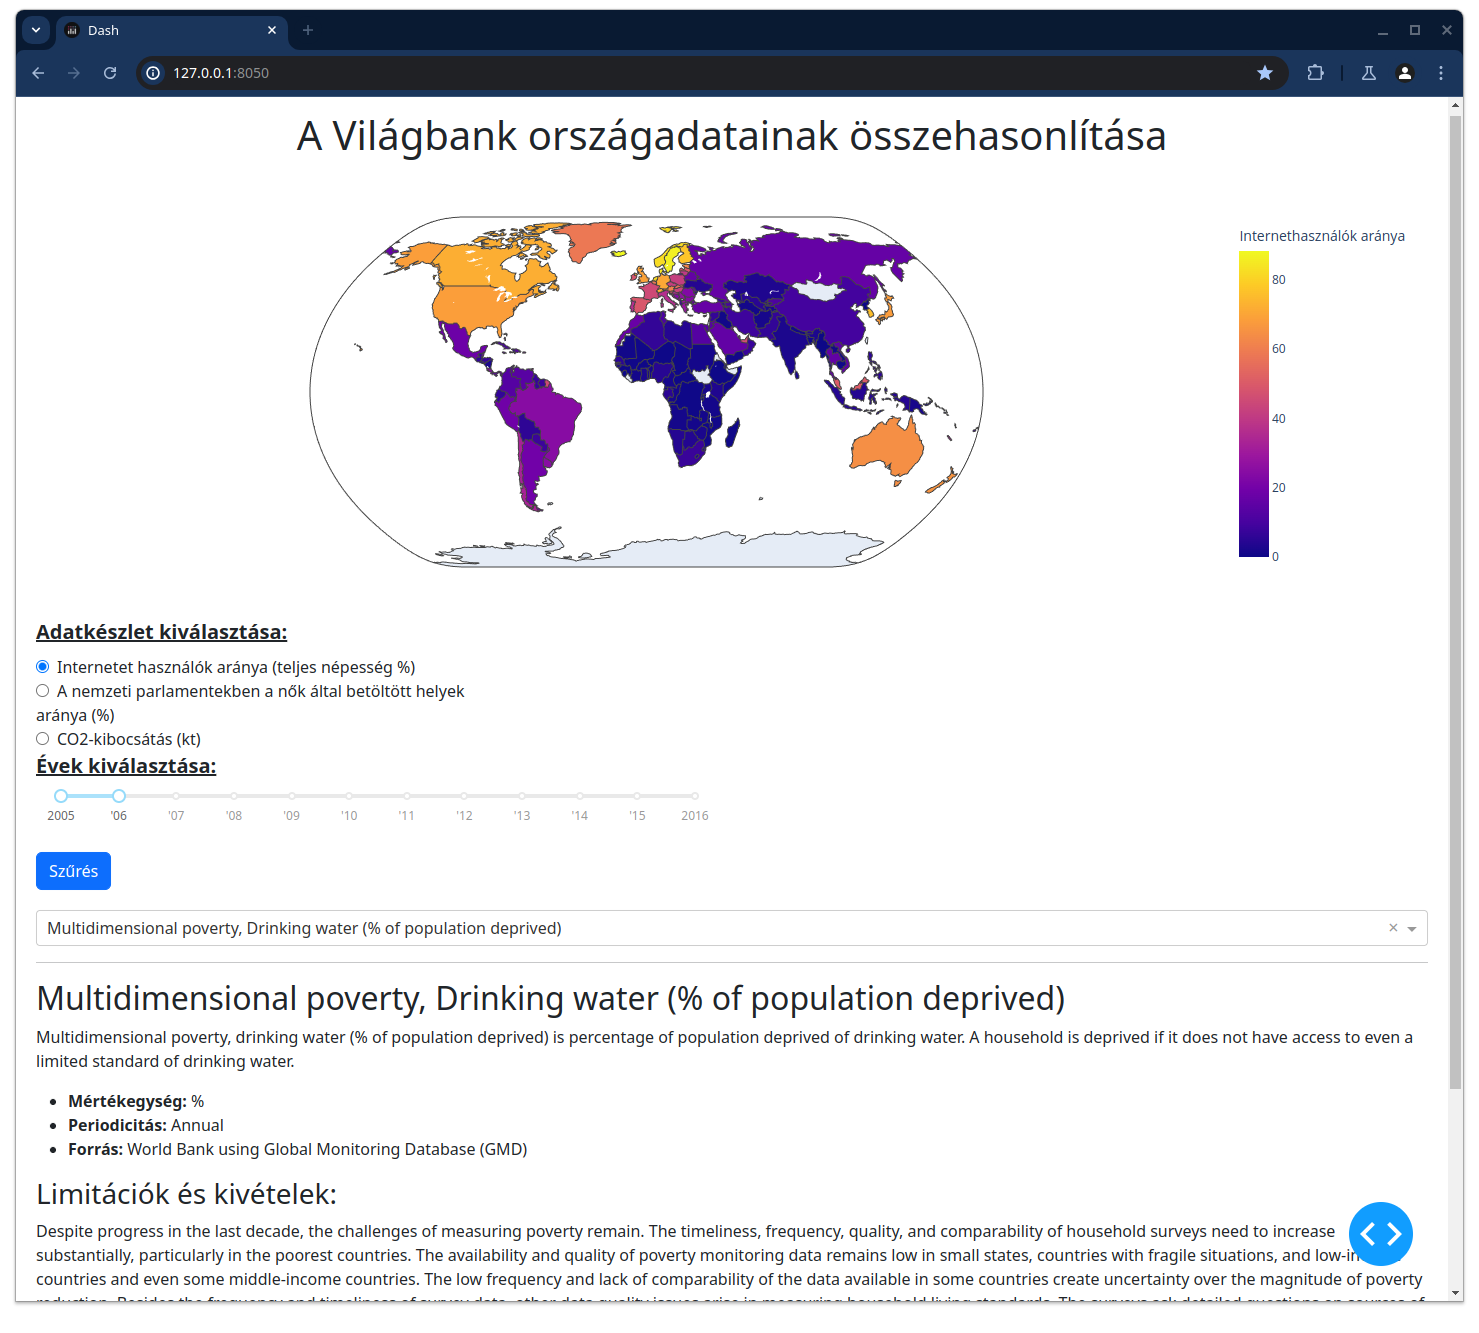
\includegraphics[width=7cm, height=7cm, keepaspectratio]{images/scatter_33.png}
				\end{center}
			\end{column}
		\end{columns}
	\end{frame}
	
	\begin{frame}{Alkalmazás térképpel és \texttt{Markdown} komponenssel (\texttt{app\_v3\_3.py})}
		\begin{center}
			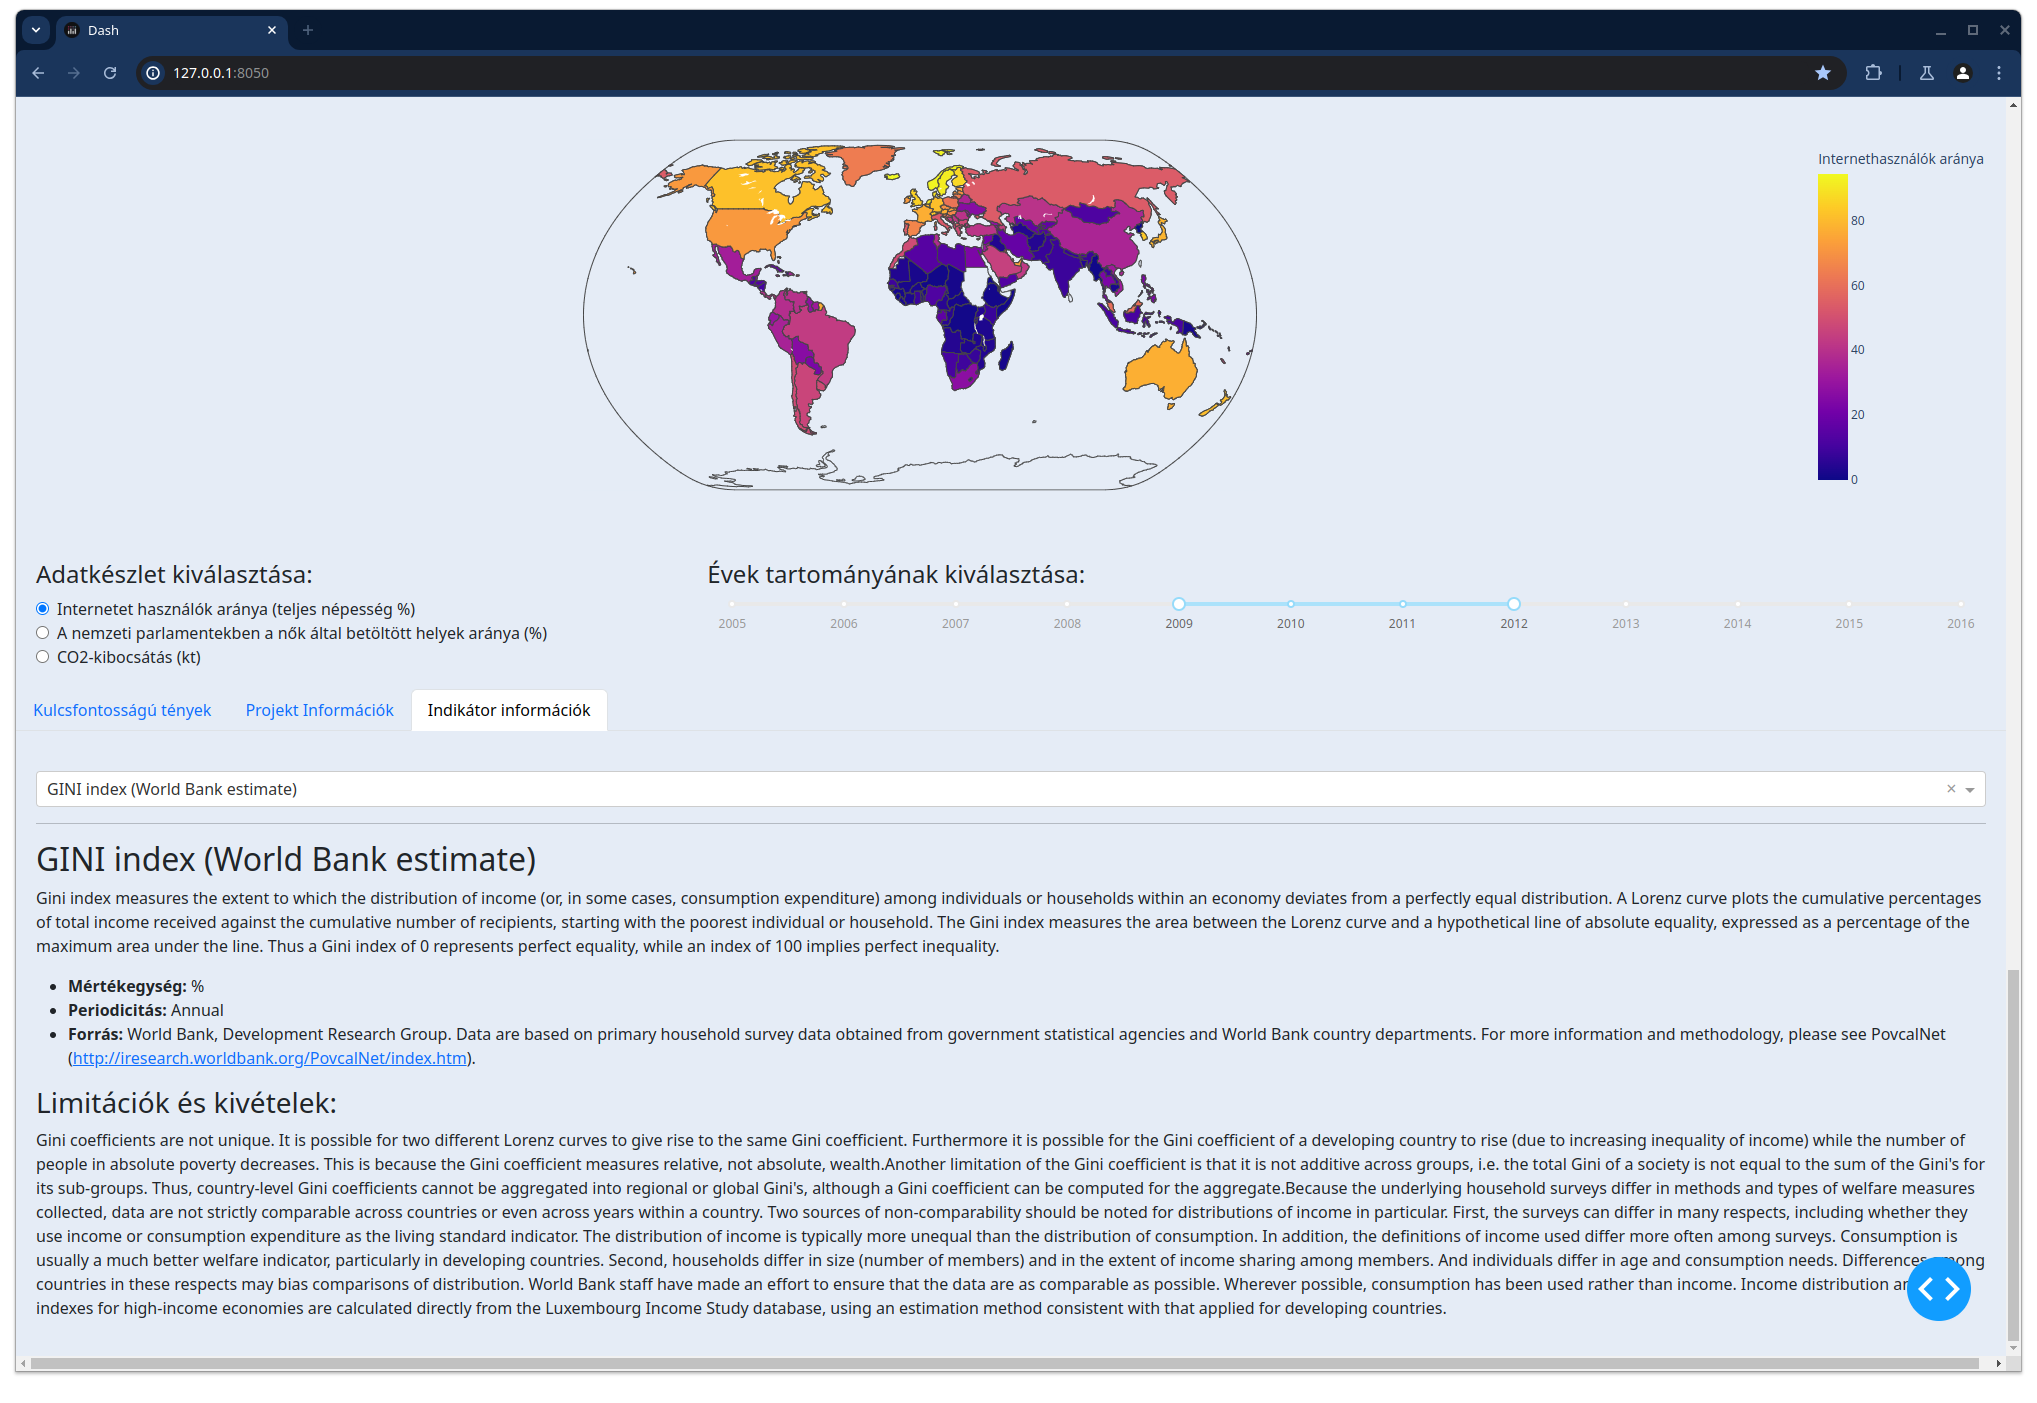
\includegraphics[width=10cm, height=7cm, keepaspectratio]{images/scatter_32.png}
		\end{center}
	\end{frame}
\end{document}